
\documentclass[11pt]{article}
\usepackage[margin=1in]{geometry}

% Core packages
\usepackage{amsmath,amssymb,amsthm}
\usepackage{graphicx}
\usepackage{tikz-cd}
\usepackage{multicol}
\usepackage[round,authoryear]{natbib}
\usepackage{hyperref}
\usepackage{comment}
\usepackage{makecell}
\usepackage{newfloat}

% Lightweight algorithm float and pseudocode environment, independent of
% algorithm/algpseudocode packages to keep the build portable.
\DeclareFloatingEnvironment[fileext=loa,listname={List of Algorithms},name=Algorithm,placement=t]{algorithm}
\SetupFloatingEnvironment{algorithm}{name=Algorithm,placement=t}
\newcounter{algline}
\newenvironment{algorithmic}
  {\begin{list}{\scriptsize\arabic{algline}:}%
     {\usecounter{algline}%
      \setlength{\leftmargin}{2em}%
      \setlength{\labelsep}{0.5em}%
      \setlength{\itemsep}{0pt}%
      \setlength{\parsep}{0pt}%
      \setlength{\topsep}{0.3em}}}%
  {\end{list}}
\newcommand{\algkw}[1]{\textbf{#1}}
\newcommand{\algIndent}{\hspace*{1.5em}}

\newtheorem{theorem}{Theorem}
\newtheorem{proposition}[theorem]{Proposition}
\newtheorem{corollary}[theorem]{Corollary}

% Paragraphs
\setlength{\parindent}{0pt}
\setlength{\parskip}{1\baselineskip}

\title{The lecture hall quadratic assignment problem}
\author{Tal Raviv}
\date{April 2026}

\begin{document}
\maketitle

\begin{abstract}
We study the post-timetabling \emph{lecture-hall assignment problem}, in which a fixed weekly timetable and realized student enrollments are given, and the decision is to assign each lecture to a compatible hall so as to minimize the walking burden imposed on students moving between consecutive lectures. The problem combines a quadratic assignment objective, driven by the product of shared enrollments and hall-to-hall distances, with interval-scheduling feasibility constraints and hall-capacity restrictions. We prove that the problem is NP-hard and that every approximation lower bound for the classical quadratic assignment problem carries over, already in a single-day, two-block special case. We develop three exact formulations---a bilinear mixed-integer quadratic program, a compact mixed-integer linear program with one auxiliary distance variable per successor pair, and a constraint-programming model---all sharing the same feasible set and admitting a natural daily decomposition. To tighten the relaxations we introduce biclique distance cuts that dominate the standard pairwise linking inequalities, together with Chv\'atal--Gomory capacity-dominance cuts and a safe compatibility-preprocessing procedure. The framework also accommodates common timetabling side constraints such as hard and soft \emph{SameRoom} and \emph{SameAttendees} requirements, for which biclique-strengthened linearizations are derived. A comprehensive numerical campaign covers daily instances derived from five large ITC~2019 competition benchmarks and from a 2023 institutional dataset from Lancaster University, whose travel-time matrix and student registrations are processed through a dedicated greedy-assignment pipeline. The compact linearized MIP emerges as the most robust formulation, and biclique strengthening is the dominant modeling device: it closes virtually all of the root-relaxation gap on both data sources and lifts the number of proven-optimal solves substantially, while cutting median solver runtimes by roughly an order of magnitude. The results demonstrate that realistically sized lecture-hall assignment instances can be solved to optimality or near-optimality within minutes, and typically within seconds, by off-the-shelf MIP technology once the biclique structure of the quadratic walking term is exploited.
\end{abstract}

\noindent\textbf{Keywords:} lecture hall assignment; quadratic assignment problem; university course timetabling; interval scheduling; mixed-integer programming; constraint programming; biclique inequalities.

\section{Introduction and background}
Universities and colleges often determine the course timetable well before they assign lectures to specific halls. Throughout this paper, we use the term \emph{hall} (or \emph{lecture hall}) to refer generically to any space used for academic activity, whether it is a traditional lecture theater, a seminar room, or a laboratory. Similarly, we use the term \emph{lecture} to refer to any scheduled academic activity, encompassing regular lectures, tutorials, or practical sessions. Once the timetable is fixed and student registration is completed, the institution knows both the enrollment in each lecture and the  enrollment overlap in between consecutive lectures. At that stage, the hall-assignment decision can have a substantial effect on student mobility across campus. Assigning consecutive lectures attended by many of the same students to distant halls may generate unnecessary walking, even when every lecture is assigned to a feasible hall. In practice, long walks between halls may also cause students to arrive late at their next lecture, thereby disrupting the beginning of lecture.  It may also be particularly challenging to students with mobility disabilities.

This observation motivates a lecture-hall assignment problem that is separate from the timetabling itself. In the lecture-hall assignment problem, the timetable, including the scheduled time interval of each lecture, is  given. The remaining task is to assign lectures to halls in a way that respects hall compatibility in terms of capacity and required facilities, while also reducing the walking burden imposed on students as they move between consecutive lectures. Other, more local, considerations may also affect the desirability of assignment of each lecture to a compatible hall, e.g., large halls are feasible but less desirable for lectures with low enrollment.   In this paper, we model this problem and present exact solution methods for it.

The proposed model is related to three main streams of literature: the quadratic assignment problem (QAP), lecture hall assignment and interval scheduling, and university course timetabling. The closest conceptual link to the QAP is the presence of pairwise interaction costs: assigning two lectures to two halls creates a cost that depends jointly on the distance between the halls and on the number of students who attend both lectures. This is analogous to the flow--distance structure that defines the classical QAP introduced by \citet{koopmans1957} and surveyed extensively by \citet{burkard1998} and \citet{loiola2007}. The QAP literature has developed a rich toolkit of solution techniques whose ideas we draw on in this paper. Classical lower bounds begin with the Gilmore--Lawler bound \citep{gilmore1962,lawler1963}, which is obtained from a linear assignment relaxation of the quadratic cost structure. Linearization-based formulations were proposed by \citet{kaufman1978}, who introduced a compact Benders-style reformulation using one auxiliary continuous variable per pair of facilities, and by \citet{frieze1983}, whose linearization exploits the permutation structure. \citet{adams1994} later developed a stronger mixed-integer linear reformulation whose linear-programming relaxation dominates earlier bounds, at the cost of a larger variable set. More recent advances include dual-based bounds derived from a Hungarian-method reformulation of the linearized model \citep{hahn1998}, semidefinite relaxations \citep{zhao1998}, lift-and-project branch-and-cut algorithms that solve increasingly tight binary relaxations on the fly \citep{burer2006}, convex quadratic reformulations and improved branch-and-bound methods \citep{anstreicher2003}, and large-scale computational studies such as \citet{anstreicher2002}, who solved previously intractable QAPLIB instances on computational grids. The same combinatorial backbone reappears in closely related facility-layout problems, for which \citet{fischer2019} develop exact branch-and-cut algorithms based on layered MIP and semidefinite relaxations and report state-of-the-art bounds on standard benchmarks. On the heuristic side, robust tabu search \citep{taillard1991} and related metaheuristics remain the dominant approach for obtaining high-quality solutions to large QAP instances. The compact linearization and the valid inequalities that we develop in Section~3 are inspired by this branch-and-cut line of work, in particular by the lift-and-project ideas of \citet{burer2006} and the layered linearization of \citet{fischer2019}, but are adapted to the combined temporal and compatibility structure of the lecture-hall setting and exploit the sparsity of the successor relation that is absent from the dense classical QAP. At the same time, the present problem differs from the standard QAP because feasibility is driven by temporal overlap, hall capacities, and the subset of lecture pairs that are consecutive on the same day.

A second relevant stream concerns lecture hall assignment and interval-based hall allocation. In this family of problems, activities with fixed or partially fixed time intervals must be assigned to halls while respecting incompatibilities caused by overlap in time. \citet{carter1992} study the lecture hall assignment problem from a complexity perspective and explicitly connect it to interval scheduling. The broader interval-scheduling literature, surveyed by \citet{kolen2007}, studies machine or resource assignment of activities with fixed time windows and provides a natural framework for the temporal-feasibility layer of our problem. In particular, the clique structure of interval graphs, which we exploit in Section~3 to tighten the overlap constraints, is a standard building block in that literature. The framework of \citet{carter1992} and \citet{kolen2007} is closely related to the feasibility component of the present model, where lectures cannot share a hall if their time intervals overlap. However, the objective considered here is richer because it is not limited to feasibility or hall utilization; instead, it introduces interaction costs across consecutive lectures through student flows and hall-to-hall distances.

A third stream is the university timetabling literature, which studies the joint allocation of courses to times and halls under institutional constraints. This is a problem which the literature refers to as the \emph{University Course Timetabling Problem.}
General surveys by \citet{schaerf1999} and \citet{burke2002} describe a broad range of formulations, including problems in which hall capacities, conflicts, and soft preferences play a central role, while the more recent review of \citet{abdipoor2023} summarizes modern meta-heuristic and hybrid approaches for university course timetabling. The field has also been shaped by three international timetabling competitions. The first competition (ITC~2002) established graph-colouring-style formulations and the first widely used benchmark set; \citet{lewis2005} illustrate the graph-grouping heuristics that dominated the early competition and provide lower bounds based on the chromatic structure of the conflict graph. The second competition \citep{mccollum2010} broadened the problem to three tracks, including curriculum-based course timetabling, for which \citet{bonutti2012} later introduced the now-standard benchmark suite, data formats, and validation protocol. The ITC~2019 competition \citep{muller2025itc2019} further generalized the model by adding rich distribution constraints and student sectioning, and produced the dataset used in our real-world campaign. On the metaheuristic side, \citet{abdullah2012} develop a tabu-based memetic approach with multiple neighbourhood structures that remains a reference point for high-quality feasible solutions on the curriculum-based competition instances. Within this literature, lecture hall assignment is often treated either as a subproblem of course timetabling or as a second-stage problem after times have been fixed. For example, \citet{torres2014} propose a two-phase approach in which course scheduling is followed by lecture hall assignment, and \citet{rappos2022} develop a mixed-integer programming model that jointly considers student allocation, hall assignment, and time-period assignment. A recent extension by \citet{davison2025} brings hybrid teaching into the university course timetabling problem by treating each lecture's delivery mode: fully online, fully in-person, or hybrid with a split of students between the two modes, as a first-class modelling element alongside the usual hall and time decisions. They formulate a multi-objective binary program that combines standard timetabling features identified from a broad literature review with new variables and constraints describing in-person versus online delivery and student mode preferences, and they solve it by a lexicographic method on benchmark data, illustrating trade-offs among demand satisfaction, hall utilisation, and hybrid-delivery quality for use in strategic decision making. Their work expands the set of constraints and objectives that a timetabling model is expected to handle but, like most models in this tradition, keeps hall assignment embedded inside the larger multi-criterion formulation rather than isolating it as a separate problem with exploitable structure. This decomposition is natural in many university settings and is also compatible with the present formulation, which assumes that the scheduled time interval of each lecture is already known.

Taken together, these three lines of literature suggest that the lecture hall assignment problem studied here combines structural ingredients that are usually treated separately. From lecture hall assignment and interval scheduling it inherits the temporal packing constraints on halls; from timetabling it inherits the academic context, capacity restrictions, and interpretation of lectures as scheduled activities; and from the QAP it inherits a pairwise objective that couples assignment decisions across lectures. A particularly close recent connection is the hall-allocation study of \citet{roomalloc2026}, who isolate the hall-assignment subproblem of the university course timetabling problem under an already-fixed weekly schedule and formulate it as a six-criterion problem with two hard constraints (hall capacity and no scheduling overlap) and four soft objectives (student relocation between buildings, mismatch between requested and assigned hall types, wasted capacity, and hall changes between consecutive lectures of the same student group). They develop customised multiobjective evolutionary algorithms augmented with problem-specific local search and constructive heuristics implemented in the jMetal framework, and benchmark them against an ILP model solved by Gurobi. The computational study uses a full-semester dataset from the University Institute of Lisbon with approximately 10{,}000 students, more than 26{,}000 scheduled lecture sessions, and over 120 lecture halls of more than 20 distinct types, and emphasises scalability and Pareto-front quality as the central performance measures.

The present framework can likewise accommodate mandatory hall features through the compatibility sets and additional hall-quality criteria through linear assignment penalties, so on the modelling surface it overlaps with four of the six criteria of \citet{roomalloc2026}. Its distinguishing features are structural and methodological. Structurally, student movement enters as a QAP-style quadratic term induced by shared enrollments and inter-hall walking distances rather than as a count of building changes or group-level hall changes; capacity and overlap are retained as hard feasibility constraints; and the remaining hall-quality criteria are combined into a single scalar objective through linear assignment penalties, which is possible because the weighting between them is under the analyst's control. Methodologically, this combined structure motivates exact mathematical-programming and constraint-programming approaches with problem-specific valid inequalities and preprocessing, rather than the multiobjective evolutionary framework favoured in \citet{roomalloc2026}. The two approaches are therefore complementary: theirs targets very large operational instances where a Pareto front among competing criteria is the primary deliverable, while ours targets a clean QAP-flavoured subproblem where exploiting pairwise structure and interval-graph cliques often yields provably optimal or near-optimal solutions.

\paragraph{Research gap and contribution.}
While the QAP literature provides powerful exact algorithms \citep{kaufman1978,frieze1983,adams1994,hahn1998,zhao1998,anstreicher2002,anstreicher2003,burer2006,fischer2019}, it assumes unrestricted assignments without temporal overlap or capacity constraints. Conversely, the timetabling and interval-scheduling literatures address these operational realities but typically rely on linear objectives or multiobjective heuristics rather than QAP-style quadratic pairwise interactions \citep{carter1992,kolen2007,lewis2005,mccollum2010,bonutti2012,abdullah2012,rappos2022,davison2025,roomalloc2026}. 

We bridge this gap by isolating the post-timetabling lecture-hall assignment problem, a setting common in institutions where course enrollments are only revealed after the schedule is set. In our framework, temporal overlap and spatial capacity act as hard constraints (with optional linear penalties for soft preferences), while the primary objective is a quadratic mapping of walking effort driven by shared student enrollments. By formally separating this subproblem, we exploit its distinct structure. We analyze its computational complexity and construct a novel, compact two-index distance-variable formulation. To strengthen this model, we introduce an easy-to-separate valid biclique inequality that shares the strength of classical lift-and-project cuts but operates in a lower dimension by leveraging the sparsity of lecture-hall compatibilities. Through comprehensive numerical studies, we demonstrate that these problem-specific mathematical-programming and constraint-programming enhancements substantially improve computational performance over baseline nonlinear formulations, solving large, realistic instances to optimality or near-optimality.

\section{Problem statement and complexity}\label{sec:problem}
We now formalize the lecture-hall assignment problem and state its complexity properties.

We consider this problem through the following sets:
\begin{description}
    \item[Halls ($H$)] Each hall $h \in H$ is defined by its capacity $u_h$, its location, and its set of available features $F_h$ (such as ``laboratory bench'', ``computer workstation'', ``projector'', or ``wheelchair-accessible entrance'').
    \item[Lectures ($L$)] Each lecture $l \in L$ is defined by its scheduled time interval, its number of registered students $s_l$, and its set of mandatory hall features $F_l^{\mathrm{req}}$ (for example, a chemistry practical must be assigned to a lab hall, and a programming session must be assigned to a hall with computer workstations).
    \item[Immediate-successor relation ($A$)] A relation $A \subseteq L \times L$, where $(l_1,l_2) \in A$ if lecture $l_2$ is scheduled immediately after lecture $l_1$ for at least one group of students.
    \end{description}

A hall $h$ is \emph{compatible} with a lecture $l$ if it has sufficient capacity and provides every mandatory feature, that is,
\[
H(l) = \{h \in H : u_h \ge s_l,\ F_l^{\mathrm{req}} \subseteq F_h\}.
\]
The compatibility set $H(l)$ is computed once from the input data and is treated as primitive in the rest of the paper. Mandatory features are deliberately handled as hard restrictions through $H(l)$ rather than as soft penalties, because in practice a chemistry practical cannot meaningfully take place in a hall without lab benches no matter what the student-flow gain would be.

The walking distance between each pair of halls $h_1, h_2 \in H$ is given by the distance matrix $d_{h_1,h_2}$. In addition, for each pair of lectures $(l_1,l_2) \in A$, we are given the number of students enrolled in both lectures, denoted by $c_{l_1,l_2}$. This number may be a simple head count or a score that gives higher weight to students with disabilities, if the institution has this information at its disposal. Finally, for each compatible lecture--hall pair $(l,h)$ with $h \in H(l)$, we are given a nonnegative \emph{assignment penalty} $p_{lh} \ge 0$ that captures local hall-quality considerations beyond the hard compatibility filter. In practice, $p_{lh}$ is constructed by aggregating several soft per-assignment effects: wasted seating capacity when a small lecture is placed in a much larger hall, absence of desirable but non-mandatory features (for example, an oversized whiteboard requested by an instructor or a preferred building wing), and institutional preferences inherited from a higher-level timetabling stage. Any such weighting is encoded by adjusting the input $p_{lh}$ before solving and does not change the formulations developed below; the relative importance of each component is therefore under the analyst's control. Together, the three ingredients $d_{h_1,h_2}$, $c_{l_1,l_2}$, and $p_{lh}$ capture the cross-lecture coupling driven by student movement and the per-assignment local quality of each hall choice.

We make the following standing assumption on the registration data.
\begin{description}
    \item[Single-lecture-at-a-time assumption]\label{asm:single-lecture} No student is registered for two lectures whose scheduled intervals overlap in time.
\end{description}
Under this assumption, every student contributes to the shared enrollment $c_{l_1,l_2}$ of a successor pair $(l_1,l_2)\in A$ at most once, and the walking-distance objective defined in the next section is well-posed on every feasible assignment. Any input that violates the assumption must be cleaned beforehand by dropping the conflicting registration from one of the two overlapping lectures; Section~\ref{subsec:Test-instances} describes one such cleaning step in our Lancaster benchmark.

The goal is to assign each lecture to a compatible hall such that no two lectures assigned to the same hall overlap in time. The objective is to minimize the sum of two terms: (i) the total walking distance traveled by students between consecutive lectures, and (ii) the total assignment penalty incurred by the chosen lecture-hall pairs. The relative weight between the two terms is implicit in the units of $c_{l_1,l_2}$ and $p_{lh}$, and is therefore controlled by the analyst when these inputs are constructed.

This problem shares features with both the quadratic assignment problem and interval scheduling, and in a sense it combines elements of both.

A natural decision version of the lecture-hall assignment problem asks whether, for a given bound $B$, there exists a feasible hall assignment whose total walking cost is at most $B$. This decision problem belongs to NP, since a proposed assignment can be verified in polynomial time by checking compatibility, non-overlap, and the resulting objective value. The next proposition states the exact and approximation hardness of the problem.

\begin{proposition}
\label{prop:hardness}
The decision version of the lecture-hall assignment problem is NP-complete, and the corresponding optimization problem is NP-hard. Moreover, for every $\rho \ge 1$, if there exists a polynomial-time $\rho$-approximation algorithm for the lecture-hall assignment problem, then there exists a polynomial-time $\rho$-approximation algorithm for the classical quadratic assignment problem (QAP). Consequently, every approximation lower bound for QAP carries over to the lecture-hall assignment problem. All of these statements remain true even for a restricted single-day case with two consecutive time blocks, identical hall capacities, and full lecture-hall compatibility.
\end{proposition}

\begin{proof}
We use a reduction from the classical QAP, which is NP-hard and inapproximable within a constant factor, see
\citet{sahni1976p,burkard1998,loiola2007}. Consider a QAP instance with facilities $\mathcal{N}=\{1,\dots,n\}$, locations $\mathcal{R}=\{1,\dots,n\}$, nonnegative flow matrix $(f_{ij})$, and nonnegative distance matrix $(d_{ab})$. First normalize the distances by setting
\[
\hat d_{aa}=0 \quad \forall a \in \mathcal{R},
\qquad
\hat d_{ab}=d_{ab}+1 \quad \forall a \neq b.
\]
For every permutation $\pi$ of the locations,
\[
\sum_{i=1}^n \sum_{j=1}^n f_{ij}\hat d_{\pi(i),\pi(j)}
=
\sum_{i=1}^n \sum_{j=1}^n f_{ij}d_{\pi(i),\pi(j)}
+
\sum_{i \neq j} f_{ij},
\]
because $\pi(i)\neq \pi(j)$ whenever $i\neq j$. Thus the normalization adds the same constant to every feasible QAP solution, so it preserves both exact comparisons and approximation ratios.

Now construct a lecture-hall instance as follows. Create $n$ halls $h_1,\dots,h_n$, all with identical capacity $u_{h_a} = U$ for some $U$ larger than every lecture size introduced below, and declare the hall feature set $F_{h_a}=\emptyset$ for every $a$. For each lecture $l$ introduced in the remainder of the construction, set the required-feature set $F_l^{\mathrm{req}}=\emptyset$ and choose a registered-students count $s_l \le U$, so that by the definition of compatibility in Section~\ref{sec:problem} every hall is compatible with every lecture. Set the assignment penalty $p_{lh}=0$ for every lecture--hall pair so that the assignment-penalty term in the objective contributes nothing. Create two sets of lectures,
\[
U=\{u_1,\dots,u_n\}
\qquad \text{and} \qquad
V=\{v_1,\dots,v_n\},
\]
where all lectures in $U$ occupy one common time block and all lectures in $V$ occupy the immediately following common time block. Every lecture in $U$ therefore overlaps every other lecture in $U$, and similarly for $V$. Since there are exactly $n$ halls, every feasible lecture-hall assignment induces two permutations of the halls: one permutation $\pi$ for the lectures in $U$ and one permutation $\sigma$ for the lectures in $V$. For every $i,j \in \{1,\dots,n\}$, include the pair $(u_i,v_j)$ in the successor set and set
\[
d_{h_a,h_b}=\hat d_{ab} \qquad \forall a,b \in \{1,\dots,n\}.
\]

Let $M$ be a positive penalty parameter, to be specified below, and define
\[
c_{u_i,v_j}=
\begin{cases}
f_{ij}+M, & \text{if } i=j,\\
f_{ij}, & \text{if } i\neq j.
\end{cases}
\]
Under a feasible lecture-hall assignment corresponding to permutations $(\pi,\sigma)$, the objective value is
\[
\sum_{i=1}^n \sum_{j=1}^n f_{ij}\hat d_{\pi(i),\sigma(j)}
+
M\sum_{i=1}^n \hat d_{\pi(i),\sigma(i)}.
\]
If $\pi\neq \sigma$, then there exists some $i$ such that $\pi(i)\neq \sigma(i)$, and therefore $\hat d_{\pi(i),\sigma(i)}\ge 1$. Hence every such assignment has value at least $M$. On the other hand, if $\pi=\sigma$, then the penalty term vanishes and the lecture-hall objective becomes
\[
\sum_{i=1}^n \sum_{j=1}^n f_{ij}\hat d_{\pi(i),\pi(j)},
\]
which is exactly the normalized QAP objective.

For the exact reduction, start from the QAP decision problem with threshold $K$ and set
\[
M = \hat K + 1, \qquad \hat K := K + \sum_{i\neq j} f_{ij}.
\]
Then any lecture-hall solution of value at most $\hat K$ must satisfy $\pi=\sigma$, and once $\pi=\sigma$ its value is exactly the normalized QAP value of the same permutation. Therefore the original QAP instance is a yes-instance if and only if the constructed lecture-hall instance admits a feasible assignment of cost at most $\hat K$. The quantity $\hat K$ is a sum of at most $n^2+1$ nonnegative integers taken directly from the QAP input, so its binary bit-length is polynomial in the bit-length of that input; consequently $M=\hat K+1$ and the resulting walking weights $c_{u_i,v_j}\in\{f_{ij},f_{ij}+M\}$ all fit in polynomially many bits, and the full lecture-hall instance is produced in polynomial time from the QAP input. Hence the construction is a Karp (polynomial-time many-one) reduction, not merely a Cook reduction, and the decision version of the lecture-hall assignment problem is NP-hard. Since it belongs to NP, it is NP-complete. Consequently, the optimization problem is NP-hard.

For the approximation statement, fix $\rho \ge 1$ and let
\[
F_{\mathrm{tot}}=\sum_{i=1}^n \sum_{j=1}^n f_{ij},
\qquad
D_{\max}=\max_{a,b\in \mathcal{R}}\hat d_{ab},
\qquad
U_{\max}=F_{\mathrm{tot}}D_{\max}.
\]
Every feasible normalized QAP solution has value at most $U_{\max}$, and therefore the optimal value $\mathrm{OPT}_{\mathrm{QAP}}$ satisfies $\mathrm{OPT}_{\mathrm{QAP}}\le U_{\max}$. Now set
\[
M=\rho U_{\max}+1.
\]
For any fixed rational $\rho\ge 1$ (equivalently, for $\rho$ given as part of the input in binary), $U_{\max}=F_{\mathrm{tot}} D_{\max}$ is a product of two nonnegative integers whose binary bit-lengths are polynomial in the QAP input, so $M$ itself has bit-length polynomial in the input and the construction of the lecture-hall instance runs in polynomial time. The approximation-preserving reduction is therefore also Karp, not merely Cook. Then every lecture-hall solution with $\pi\neq \sigma$ has value at least
\[
M=\rho U_{\max}+1 > \rho U_{\max}\ge \rho\,\mathrm{OPT}_{\mathrm{QAP}}.
\]
But the optimal lecture-hall value is exactly $\mathrm{OPT}_{\mathrm{QAP}}$, attained by solutions with $\pi=\sigma$. Therefore any polynomial-time $\rho$-approximation algorithm for the lecture-hall assignment problem, applied to this constructed instance, must return a solution with $\pi=\sigma$, because every solution with $\pi\neq \sigma$ already exceeds $\rho$ times the optimum. For such a returned solution, the lecture-hall objective is exactly the normalized QAP objective of the same permutation. Hence a polynomial-time $\rho$-approximation for the lecture-hall assignment problem yields a polynomial-time $\rho$-approximation for QAP.

Thus both exact hardness and approximation hardness follow from the same reduction family.
\end{proof}

\begin{corollary}
\label{cor:no-constant-approx}
Unless $\mathrm{P}=\mathrm{NP}$, there is no polynomial-time constant-factor approximation algorithm for the lecture-hall assignment problem. The same inapproximability holds even when the input is restricted to a single-day instance with two consecutive time blocks, identical hall capacities, and full lecture-hall compatibility.
\end{corollary}
\begin{proof}
\citet{sahni1976p} proved that, unless $\mathrm{P}=\mathrm{NP}$, no polynomial-time algorithm approximates the classical QAP within any constant factor. By Proposition~\ref{prop:hardness}, any polynomial-time $\rho$-approximation algorithm for the lecture-hall assignment problem would, for the same $\rho$, yield a polynomial-time $\rho$-approximation for QAP. The reduction in the proof of Proposition~\ref{prop:hardness} uses only a single day, two consecutive time blocks, identical hall capacities, and full compatibility, so the inapproximability transfers verbatim to that restricted input class.
\end{proof}


\section{Models and algorithms}
This section presents three complementary exact modeling views of the lecture-hall assignment problem. We begin with a natural mixed-integer quadratic programming formulation, then derive a compact mixed-integer linear programming reformulation, and finally present a constraint-programming formulation that captures the assignment structure directly. All three base formulations optimize the same combined objective from Section~\ref{sec:problem}: the quadratic walking term weighted by shared enrollments and hall-to-hall distances, plus the linear assignment-penalty term $\sum_l p_{l,a_l}$. After these three base formulations, we describe several modeling improvements that can be layered on top of them, including valid inequalities, biclique cuts, and safe compatibility preprocessing.

For notational convenience, define
\[
A' = \{(l_1,l_2) \in A : c_{l_1,l_2} > 0\}.
\]

\subsection{Mixed-Integer Quadratic Programming Formulation}
\label{subsec:miqp-formulation}
A natural mixed-integer quadratic programming (MIQP) formulation is as follows. For each lecture $l \in L$ and each compatible hall $h \in H(l)$, let
\begin{equation}
    x_{lh} =
    \begin{cases}
        1 & \text{if lecture $l$ is assigned to hall $h$,}\\
        0 & \text{otherwise.}
    \end{cases}
    \label{eq:nlp-x-def}
\end{equation}
Recall that $s_l$ is the number of students attending lecture $l$, $u_h$ is the capacity of hall $h$, and $H(l) \subseteq H$ is the compatibility set defined in Section~\ref{sec:problem} that respects both the capacity bound $u_h \ge s_l$ and the mandatory-feature inclusion $F_l^{\mathrm{req}} \subseteq F_h$. Fix a day $d \in D$, and define the interval graph $G_d=(L_d,E_d)$ in which two lectures are adjacent if and only if their scheduled intervals overlap. Since lecture intervals lie on a line, $G_d$ is an interval graph. Let $\mathcal{C}_d$ denote the family of maximal cliques of $G_d$. The problem can then be written as
\begin{align}
    \min \quad & \sum_{(l_1,l_2) \in A'} c_{l_1,l_2} \, \sum_{h_1 \in H(l_1)} \sum_{h_2 \in H(l_2)}  d_{h_1,h_2} \, x_{l_1 h_1} x_{l_2 h_2}
    + \sum_{l \in L} \sum_{h \in H(l)} p_{lh}\, x_{lh} \label{eq:nlp-obj} \\
    \text{s.t.} \quad
    & \sum_{h \in H(l)} x_{lh} = 1, && \forall l \in L, \label{eq:nlp-assign} \\
    & \sum_{l \in C:\, h \in H(l)} x_{lh} \le 1, && \forall d \in D,\ \forall C \in \mathcal{C}_d,\ \forall h \in H, \label{eq:nlp-overlap} \\
    & x_{lh} \in \{0,1\}, && \forall l \in L,\ \forall h \in H(l). \label{eq:nlp-binary}
\end{align}
The objective has two parts. The first is quadratic: the walking cost of assigning a lecture to a hall depends on where the immediately succeeding lecture is assigned, and each contribution is scaled by the shared-enrollment weight $c_{l_1,l_2}$. The second is linear: each compatible lecture--hall pair $(l,h)$ contributes its local assignment penalty $p_{lh}$ whenever it is selected. The first set of constraints ensures that each lecture is assigned to exactly one compatible hall, and the second enforces non-overlap by requiring that, for every hall and every maximal clique of mutually overlapping lectures, at most one lecture in that clique may use the hall.

An immediate structural observation is that the problem is separable by day. Let $D$ denote the set of teaching days, and let $T$ denote the set of time units used to describe lecture intervals. For each $d \in D$, let $L_d \subseteq L$ be the set of lectures scheduled on day $d$, and let $A_d \subseteq A$ be the set of successor pairs whose two lectures both belong to day $d$. For each time unit $t \in T$, let $L(t) \subseteq L$ denote the set of lectures whose scheduled interval contains $t$, so that $L(t)$ is the set of vertices of the interval graph $G_d$ active at $t$ (with $d$ the day that contains $t$). Because temporal-overlap constraints involve only lectures that occur on the same day, and because an immediate-successor pair must also lie within a single day, both the objective and feasibility constraints decompose across days. Therefore, the weekly problem can be written as the sum of independent daily subproblems,
\begin{equation}
    \min \sum_{d \in D} f_d(x^d),
\end{equation}
where each $f_d$ is the objective induced by the lectures and successor pairs of day $d$, and $x^d$ denotes the hall-assignment decisions for that day. In particular, solving the overall weekly problem is equivalent to solving one independent lecture-hall assignment problem for each day and combining the resulting assignments. This observation is useful both computationally and conceptually. Therefore, in what follows one may interpret the model as applying either to the full week or, equivalently, to a single-day instance.

\subsection{Mixed-Integer Programming Reformulation}
\label{subsec:milp-formulation}
A compact linearization can be obtained by introducing, for each successor pair $(l_1,l_2) \in A$ such that $c_{l_1,l_2} > 0$, one nonnegative continuous variable $z_{l_1 l_2}$ representing the realized hall-to-hall distance induced by that pair. The linear assignment-penalty term is already linear in the $x$ variables and so is transferred verbatim from \eqref{eq:nlp-obj}. The problem can then be reformulated as the mixed-integer linear program
\begin{align}
    \min \quad & \sum_{(l_1,l_2) \in A'} c_{l_1,l_2}\, z_{l_1 l_2}
    + \sum_{l \in L} \sum_{h \in H(l)} p_{lh}\, x_{lh} \label{eq:milp-obj} \\
    \text{s.t.}  \quad &   \text{Constraints \eqref{eq:nlp-assign} and \eqref{eq:nlp-overlap}} \nonumber\\
   & z_{l_1 l_2} \ge d_{h_1,h_2}\bigl(x_{l_1 h_1} + x_{l_2 h_2} - 1\bigr), && \forall (l_1,l_2) \in A',  h_1 \in H(l_1), h_2 \in H(l_2), \label{eq:milp-link3} \\
   & x_{lh} \in \{0,1\}, && \forall l \in L,\ \forall h \in H(l), \label{eq:milp-x-binary} \\
    & z_{l_1 l_2} \ge 0, && \forall (l_1,l_2) \in A'. \label{eq:milp-z-nonneg}
\end{align}
This reformulation is exact. The linear assignment-penalty term is the same expression as in the MIQP model and therefore needs no further argument. For the quadratic walking term, since each lecture is assigned to exactly one hall, for every pair $(l_1,l_2)$ there is exactly one compatible hall pair $(h_1,h_2)$ for which $x_{l_1 h_1}=x_{l_2 h_2}=1$; for that pair, constraint~\eqref{eq:milp-link3} yields
\[
z_{l_1 l_2} \ge d_{h_1,h_2}.
\]
For every other compatible hall pair $(h'_1,h'_2)\neq (h_1,h_2)$, at least one of $x_{l_1 h'_1}$ and $x_{l_2 h'_2}$ equals zero, so the bracket $x_{l_1 h'_1}+x_{l_2 h'_2}-1$ is nonpositive; combined with $d_{h'_1,h'_2}\ge 0$, the right-hand side of \eqref{eq:milp-link3} is then at most zero and the corresponding constraint is already implied by the nonnegativity bound $z_{l_1 l_2} \ge 0$. Therefore, because the objective minimizes $\sum c_{l_1,l_2} z_{l_1 l_2}$ with $c_{l_1,l_2}\ge 0$ and $z_{l_1 l_2}\ge 0$, the optimal value of $z_{l_1 l_2}$ is exactly the realized distance $d_{h_1,h_2}$ associated with the halls assigned to $l_1$ and $l_2$. Multiplying by $c_{l_1,l_2}$ in the objective recovers the original walking-cost contribution. Restricting the $z$ variables to pairs with $c_{l_1,l_2} > 0$ is sufficient, since pairs with zero shared enrollment do not contribute to the walking part of the objective, and the assignment-penalty part is independent of $z$.

Compared with the standard disaggregated linearization that introduces one variable for each tuple $(l_1,l_2,h_1,h_2)$, formulation \eqref{eq:milp-obj}--\eqref{eq:milp-z-nonneg} is substantially more compact in the number of additional variables. In addition, placing the shared-enrollment weight $c_{l_1,l_2}$ in the objective rather than in the linking constraints yields a better-scaled coefficient matrix while preserving the exact same optimal assignment. The hall-capacity side is also written in compact form, since the feasibility constraints are imposed only for maximal cliques of the interval graph rather than for every time step separately. However, this compactness does not necessarily imply a stronger linear-programming relaxation on the linking side.
Strengthening inequalities for this compact reformulation, and their CP analogues, are described in Subsection~\ref{subsec:Modeling-improvements}.

\subsection{Constraint Programming Formulation}
\label{subsec:cp-formulation}
A constraint-programming (CP) formulation captures the assignment structure more directly by replacing the binary assignment variables with one integer decision variable $a_l$ for each lecture $l \in L$, whose domain is restricted to the compatible set $H(l)$. Because CP-SAT operates natively on integer variables with finite domains, the walking distance and the per-lecture assignment penalty are not passed to the solver as symbolic expressions $d_{a_{l_1},a_{l_2}}$ and $p_{l, a_l}$, but as auxiliary integer variables tied to the hall assignments through extensional (tuple-table) constraints. Specifically, for each lecture $l \in L$ introduce a nonnegative integer variable
\[
q_l \in \bigl\{\, p_{lh} : h \in H(l) \,\bigr\}
\]
that records the realized assignment penalty, and for each successor pair $(l_1,l_2) \in A'$ introduce a nonnegative integer variable
\[
z_{l_1 l_2} \in \bigl\{\, d_{h_1,h_2} : h_1 \in H(l_1),\ h_2 \in H(l_2) \,\bigr\}
\]
that records the realized hall-to-hall walking distance. The CP model is then
\begin{align}
    \min \quad & \sum_{(l_1,l_2) \in A'} c_{l_1,l_2}\, z_{l_1 l_2}
    + \sum_{l \in L} q_l \label{eq:cpsat-obj} \\
    \text{s.t.} \quad
    & a_l \in H(l), && \forall l \in L, \label{eq:cpsat-domain} \\
    & (a_l,\, q_l) \in \bigl\{\, (h,\, p_{lh}) : h \in H(l) \,\bigr\}, && \forall l \in L, \label{eq:cpsat-q-table} \\
    & (a_{l_1},\, a_{l_2},\, z_{l_1 l_2}) \in \bigl\{\, (h_1,\, h_2,\, d_{h_1,h_2}) : h_1 \in H(l_1),\ h_2 \in H(l_2) \,\bigr\},
    && \forall (l_1,l_2) \in A', \label{eq:cpsat-z-table} \\
    & \text{AllDifferent}\bigl(\{\, a_l : l \in L(t) \,\}\bigr), && \forall t \in T. \label{eq:cpsat-alldiff}
\end{align}
The objective~\eqref{eq:cpsat-obj} sums, over successor pairs with positive shared enrollment, the weight $c_{l_1,l_2}$ times the realized walking distance $z_{l_1 l_2}$, plus the per-lecture assignment penalty $q_l$. Constraint~\eqref{eq:cpsat-domain} encodes the hard feasibility requirements entirely through the domain of $a_l$: the capacity bound $u_h \ge s_l$ and the feature inclusion $F_l^{\mathrm{req}} \subseteq F_h$ are already built into the CP decision variable via the compatibility set $H(l)$, so no separate assignment equalities or overlap-by-hall inequalities are needed. Constraints~\eqref{eq:cpsat-q-table} and~\eqref{eq:cpsat-z-table} are the tuple-table encodings of the relations $q_l = p_{l, a_l}$ and $z_{l_1 l_2} = d_{a_{l_1}, a_{l_2}}$, respectively: each hall (or compatible hall pair) contributes one tuple that pairs the hall configuration with its induced penalty or distance value, so the auxiliary variable is pinned by the choice of $a$ as soon as the relevant hall domain values are fixed. Constraint~\eqref{eq:cpsat-alldiff} enforces temporal feasibility: for every time unit $t$, all lectures active during that time must take distinct hall values, so no hall is used simultaneously by two overlapping lectures.

Our OR-Tools CP-SAT implementation posts both tuple-table relations through the \texttt{AddAllowed\-Assignments} API, which takes an ordered list of integer variables together with the explicit list of allowed tuples shown in~\eqref{eq:cpsat-q-table} and~\eqref{eq:cpsat-z-table}. We prefer this explicit tabular encoding to an \texttt{AddElement}-based alternative for two reasons. First, \texttt{AddAllowed\-Assignments} directly represents the joint relation between a pair of index variables and the looked-up value in a single constraint, whereas \texttt{AddElement} indexes a fixed one-dimensional array by a single integer variable and therefore does not express the two-index distance lookup $z_{l_1 l_2} = d_{a_{l_1},a_{l_2}}$ without auxiliary intermediate variables. Second, the tuple tables list only halls (or hall pairs) that belong to the compatibility sets, so after the preprocessing of Subsection~\ref{subsec:Modeling-improvements} the distance table for pair $(l_1,l_2)$ has size exactly $|H(l_1)|\cdot|H(l_2)|$, and no infeasible $(h_1,h_2)$ combination is ever enumerated. As in the MIP reformulation of Subsection~\ref{subsec:milp-formulation}, it is enough to materialize $z_{l_1 l_2}$ only for pairs $(l_1,l_2) \in A'$, since pairs with zero shared enrollment do not contribute to the walking part of the objective.

\subsection{Modeling improvements}  \label{subsec:Modeling-improvements}
Several enhancements can be layered on top of the three base formulations without changing the underlying problem. Some of them are common to all three modeling views, while others are specific to the compact MIP reformulation and its CP analogue.

\paragraph{Capacity-dominance cuts.}
A first general improvement combines the hall-capacity structure with the clique-overlap restriction. For each day $d \in D$, each maximal clique $C \in \mathcal{C}_d$, and each capacity threshold $\kappa \ge 0$, define the sets
\[
L_\kappa(C)=\{\,l \in C : s_l > \kappa\,\}, \qquad
H_\kappa=\{\,h \in H : u_h > \kappa\,\}.
\]
Every lecture $l \in L_\kappa(C)$ has $H(l) \subseteq H_\kappa$ by the capacity definition, so all of its assignment mass is placed on halls in $H_\kappa$. Summing the clique-overlap inequalities~\eqref{eq:nlp-overlap} over $h \in H_\kappa$ and isolating the contribution of the large lectures yields the \emph{capacity-dominance cut}
\begin{equation}
    \sum_{l \in C \setminus L_\kappa(C)}\ \sum_{h \in H(l) \cap H_\kappa} x_{lh}
    \;\le\; |H_\kappa| - |L_\kappa(C)|,
    \qquad \forall d \in D,\ \forall C \in \mathcal{C}_d,\ \forall \kappa \ge 0.
    \label{eq:capacity-dominance}
\end{equation}
Because $|L_\kappa(C)|$ and $|H_\kappa|$ depend only on the input data, the cut is an explicit linear inequality in the assignment variables whose right-hand side is a pre-computed nonnegative integer. It states that once the $|L_\kappa(C)|$ largest lectures of the clique have claimed their share of the $|H_\kappa|$ halls whose capacity exceeds $\kappa$, the remaining lectures in $C$ may collectively occupy at most $|H_\kappa|-|L_\kappa(C)|$ of the large halls. Only threshold values $\kappa$ that coincide with distinct hall capacities need to be instantiated, so the family contains at most $|\mathcal{C}_d| \cdot |\{u_h : h \in H\}|$ inequalities per day. The cut is a Chv\'atal--Gomory consequence of~\eqref{eq:nlp-assign}--\eqref{eq:nlp-overlap} and is therefore valid for every integer-feasible solution of the MIQP, MIP, and CP formulations alike. In the MIQP and MIP formulations it can be added directly as a linear inequality in the assignment variables. In the CP formulation it can be represented by Boolean indicators that record whether a lecture is assigned to a hall in $H_\kappa$, followed by the corresponding redundant upper bound on the sum of those indicators. If preprocessing is applied beforehand, the cut can be posted on the reduced compatibility sets without modification.

\paragraph{Biclique cuts.}
The next family of improvements is specific to the compact MIP reformulation. Fix a pair $(l_1,l_2) \in A'$  and  a pair of halls  $h_1 \in H(l_1)$ and $h_2 \in H(l_2)$, let $S_1 \subseteq H(l_1)$ and $S_2 \subseteq H(l_2)$  such that $d_{h'_1,h'_2} \ge d_{h_1,h_2} $ for every $h'_1 \in S_1$ and $h'_2 \in S_2$. Then the following inequality is valid:
\begin{equation}
    z_{l_1 l_2} \ge d_{h_1,h_2}\!\left(\sum_{h'_1 \in S_1} x_{l_1 h'_1} + \sum_{h'_2 \in S_2} x_{l_2 h'_2} - 1\right),
    \qquad \forall (l_1,l_2) \in A', h_1 \in H(l_1), h_2  \in H(l_2) .
    \label{eq:milp-link-biclique}
\end{equation}
If the assigned hall of $l_1$ lies in $S_1$ and that of $l_2$ lies in $S_2$, then both summations equal 1 and \eqref{eq:milp-link-biclique} forces $z_{l_1 l_2} \ge d_{h_1,h_2}$, which is correct since the realized distance is at least $d_{h_1,h_2}$. Otherwise the right-hand side is nonpositive and the cut is implied by the nonnegativity of $z_{l_1 l_2}$. The basic constraints \eqref{eq:milp-link3} are the special case $S_1 = \{h_1\}$ and $S_2 = \{h_2\}$; taking larger bicliques yields strictly stronger cuts that can separate fractional solutions satisfying all pairwise constraints.

In practice we generate a family of patterns $(S_1, S_2, \delta)$ by the anchor-based procedure in Algorithm~\ref{alg:biclique}. For each anchor pair $(h_1,h_2) \in H(l_1) \times H(l_2)$ the algorithm sets the common threshold $\delta = d_{h_1,h_2}$, expands $S_2$ to every hall in $H(l_2)$ at distance at least $\delta$ from the anchor $h_1$, and then expands $S_1$ to every hall in $H(l_1)$ at distance at least $\delta$ from every element of $S_2$. The anchor itself always satisfies $h_1 \in S_1$ and $h_2 \in S_2$, so \eqref{eq:milp-link-biclique} evaluated at the returned triple is at least as strong as the base pair-distance constraint obtained from the same anchor. Distinct anchors often produce the same triple, which is why the generated patterns are deduplicated before any cut is posted. For every returned triple $(S_1,S_2,\delta)$ we add one inequality of the form~\eqref{eq:milp-link-biclique} with $d_{h_1,h_2}$ replaced by $\delta$, so the total number of biclique cuts posted for a successor pair is bounded by $|H(l_1)| \cdot |H(l_2)|$ and in practice is substantially smaller because of the deduplication. In the CP model of Subsection~\ref{subsec:cp-formulation}, the same logic is translated into propagation constraints enforcing lower bounds on the auxiliary variables $z_{l_1 l_2}$ whenever the two assigned halls fall into the corresponding threshold sets.

\begin{algorithm}[t]
\caption{Biclique distance patterns for a successor pair $(l_1,l_2) \in A'$.}
\label{alg:biclique}
\hrule height 0.8pt
\vspace{0.3em}
\textbf{Input:} compatibility sets $H(l_1)$, $H(l_2)$, hall-to-hall distance matrix $d$. \\
\textbf{Output:} deduplicated set $\mathcal{P}(l_1,l_2)$ of patterns $(S_1,S_2,\delta)$.
\hrule height 0.4pt
\begin{algorithmic}
\item $\mathcal{P}(l_1,l_2) \gets \emptyset$
\item \algkw{for each} $(h_1,h_2) \in H(l_1) \times H(l_2)$ \algkw{do}
\item \algIndent $\delta \gets d_{h_1,h_2}$
\item \algIndent $S_2 \gets \{\, h \in H(l_2) : d_{h_1,h} \ge \delta \,\}$
\item \algIndent $S_1 \gets \{\, h \in H(l_1) : d_{h,h''} \ge \delta \text{ for every } h'' \in S_2 \,\}$
\item \algIndent $\mathcal{P}(l_1,l_2) \gets \mathcal{P}(l_1,l_2) \cup \{(S_1,S_2,\delta)\}$
\item \algkw{end for}
\item \algkw{return} $\mathcal{P}(l_1,l_2)$
\end{algorithmic}
\vspace{-0.3em}
\hrule height 0.8pt
\end{algorithm}

\paragraph{Compatibility preprocessing.}
A final improvement shrinks the compatibility sets $H(l)$ before solving any of the three formulations. Fix a target lecture $l' \in L$ and consider the auxiliary problem
\begin{align*}
    U_{l'} = \max \quad & \sum_{h \in H(l')} u_h x_{l'h} \\
    \text{s.t.} \quad
    & \sum_{h \in H(l)} x_{lh} = 1, && \forall l \in L, \nonumber\\
    & \sum_{l \in C:\, h \in H(l)} x_{lh} \le 1, && \forall d \in D,\ \forall C \in \mathcal{C}_d,\ \forall h \in H, \nonumber\\
    & x_{lh} \in \{0,1\}, && \forall l \in L,\ \forall h \in H(l). \nonumber
\end{align*}
This model keeps only the hard feasibility constraints and maximizes the capacity assigned to the single lecture $l'$. If $U_{l'}$ denotes its optimal value, then every hall $h \in H(l')$ with $u_h > U_{l'}$ may be removed from $H(l')$. Indeed, suppose that some globally feasible assignment uses lecture $l'$ in a hall $\hat h$ with $u_{\hat h} > U_{l'}$. That same assignment satisfies the preprocessing constraints above and attains objective value at least $u_{\hat h}$, contradicting the definition of $U_{l'}$. Therefore the reduced set
\[
\widehat H(l') = \{h \in H(l') : u_h \le U_{l'}\}
\]
preserves all feasible solutions of the original problem. Applying this optimization once to every lecture yields one valid global reduction pass for the MIQP, the compact MIP, and the CP model alike. Moreover, the pass can be repeated on the reduced compatibility sets. The iteration is monotone in the following sense: removing a hall from $H(l'')$ for any lecture $l''$ can only shrink the feasible region of the auxiliary problem for every other target lecture $l'$, since one of the candidate assignments for $l''$ simply becomes unavailable. Hence $U_{l'}$ is non-increasing from one round to the next, and consequently $\widehat H(l')$ is non-increasing as well. Each round therefore preserves the feasible set of the preceding reduced model, the sequence of compatibility sets shrinks monotonically, and the iteration terminates at a fixed point after at most $\sum_{l \in L} |H(l)|$ rounds. In the MIQP and MIP formulations, this directly removes assignment variables and all associated overlap and linking constraints. In the CP model, it shrinks the domains of the assignment variables and reduces the size of the distance tables or element encodings. In practice, the preprocessing used in our implementation is exactly this fixed-point procedure.

One may also use a cheaper lightweight version. Let
\[
L'(l') = \{l'\} \cup \{l \in L : \text{$l$ overlaps $l'$ in time}\},
\]
and solve the same maximization problem with $L'(l')$ replacing $L$ and with the overlap constraints restricted accordingly. Let its optimal value be $\widetilde U_{l'}$. To see that this is a valid relaxation, note that any feasible solution $x$ of the full auxiliary problem, when projected to the variables indexed by $L'(l')$, still satisfies every assignment constraint of $L'(l')$ and every overlap constraint restricted to $L'(l')$: dropping the nonnegative terms contributed by lectures outside $L'(l')$ from the left-hand side of a $\le 1$ inequality can only weaken it. Since the lightweight objective depends only on $x_{l',h}$ and the projection preserves its value,
\[
\widetilde U_{l'} \ge U_{l'}.
\]
Consequently, deleting from $H(l')$ only the halls with capacity larger than $\widetilde U_{l'}$ is still safe: it may leave more halls than the full preprocessing, but it cannot remove a hall that is needed by a globally feasible solution. As in the full version, one may apply the lightweight reduction repeatedly until a fixed point is reached. The same monotonicity argument carries over: shrinking $H(l'')$ for any lecture $l''$ can only tighten the lightweight auxiliary problem for $l'$ in the next round, so $\widetilde U_{l'}$ is non-increasing across rounds and the iteration terminates at a fixed point.

\subsection{SameRoom and SameAttendees side constraints}
Capacity limits, mandatory hall features, and soft per-assignment preferences are already part of the base model through the compatibility set $H(l)$ and the penalty coefficients $p_{lh}$ defined in Section~\ref{sec:problem}. However, the timetabling literature also considers pairwise side constraints that couple the hall choices of two different lectures, and these cannot be encoded through $H(l)$ or $p_{lh}$ alone. In this subsection we show how the two most common such constraints from the ITC 2019 competition model \citep{muller2025itc2019}, \emph{SameRoom} and \emph{SameAttendees}, are accommodated by the three formulations of Sections~3.1--3.3, in both their hard and soft forms.

The \emph{SameRoom} constraint requires two lectures, scheduled at non-overlapping times, to be assigned to the same hall. It can be formulated either as a hard constraint that must be satisfied by every feasible solution or as a soft constraint with an associated violation penalty.
Let $C_1^{hard}$ be the set of lecture pairs for which a hard SameRoom constraint is imposed. Then the following MIP and MIQP constraints express it:
\begin{equation}
	\label{eq:hard-SameRoom} x_{l_1,h} = x_{l_2,h}     \qquad \forall (l_1,l_2) \in C_1^{hard}, h \in H(l_1) \cap H(l_2),
\end{equation}
and for the CP formulation it is even more straightforward:
\begin{equation}
	\label{eq:hard-SameRoom-CP} a_{l_1} = a_{l_2}     \qquad \forall (l_1,l_2) \in C_1^{hard}
\end{equation}

In the hard case, the compatible hall sets of the two lectures can be reduced to the intersection of their original feasible sets, that is,
\[
H'(l_1)=H'(l_2)=H(l_1) \cap H(l_2).
\]

Alternatively, suppose that SameRoom is a soft constraint for a pair of lectures $l_1,l_2$, with penalty $\pi_{l_1,l_2}$ if the two lectures are assigned to different halls. Let $C_1^{soft}$ be the set of such pairs, and for each pair introduce a binary variable $v_{l_1,l_2}$ that equals $1$ when the constraint is violated. A linear encoding for the MIP formulation is
\begin{equation}
	\label{eq:soft-SameRoom-a} v_{l_1,l_2} \ge x_{l_1,h} - x_{l_2,h} \qquad \forall (l_1,l_2) \in C_1^{soft},\ h \in H(l_1) \cap H(l_2),
\end{equation}
\begin{equation}
	\label{eq:soft-SameRoom-b} v_{l_1,l_2} \ge x_{l_2,h} - x_{l_1,h} \qquad \forall (l_1,l_2) \in C_1^{soft},\ h \in H(l_1) \cap H(l_2),
\end{equation}
\begin{equation}
	\label{eq:soft-SameRoom-c} v_{l_1,l_2} \ge x_{l_1,h} \qquad \forall (l_1,l_2) \in C_1^{soft},\ h \in H(l_1)\setminus H(l_2),
\end{equation}
\begin{equation}
	\label{eq:soft-SameRoom-d} v_{l_1,l_2} \ge x_{l_2,h} \qquad \forall (l_1,l_2) \in C_1^{soft},\ h \in H(l_2)\setminus H(l_1).
\end{equation}
The corresponding penalty term
\[
\sum_{(l_1,l_2) \in C_1^{soft}} \pi_{l_1,l_2} v_{l_1,l_2}
\]
is then added to the objective function. In the MIQP formulation, one may avoid the auxiliary variables entirely and add the direct bilinear penalty
\[
\sum_{(l_1,l_2) \in C_1^{soft}} \pi_{l_1,l_2}
\left(
1-\sum_{h \in H(l_1)\cap H(l_2)} x_{l_1h}x_{l_2h}
\right).
\]
Because each lecture is assigned to exactly one hall, the inner sum equals $1$ if and only if the two lectures use the same compatible hall, and equals $0$ otherwise, so this term is exactly the SameRoom violation penalty. Implementation of the soft SameRoom constraint in the CP model is more straightforward: one may simply add the term
\[
\sum_{(l_1,l_2) \in C_1^{soft}} \pi_{l_1,l_2}\,[a_{l_1} \ne a_{l_2}]
\]
using a reification construct that evaluates to $1$ when the logical condition is true and to $0$ otherwise.

An important caveat is that SameRoom constraints, in both their hard and soft forms, are typically defined over the full weekly timetable. For example, a lecture given on Monday may be required to use the same hall as a related lecture given on Wednesday. If such cross-day constraints are enforced, the problem is no longer decomposable by day, and one must solve at least the whole week, and possibly the whole term, simultaneously.

Another common timetabling side constraint that is also relevant here, albeit in a more restricted sense, is \emph{SameAttendees} \citep{muller2025itc2019}. In the timetabling model, this constraint limits the travel time between two lectures that may share students. In our setting, where event times are fixed in advance, it becomes a restriction on the admissible hall pairs for two given lectures. Let $C_2^{hard}$ be the set of lecture pairs with a hard SameAttendees constraint, and let
\[
F_{l_1,l_2} \subseteq H(l_1)\times H(l_2)
\]
denote the set of forbidden hall pairs for a given pair $(l_1,l_2)$. If $l_1$ ends before $l_2$ starts, then $(h_1,h_2)\in F_{l_1,l_2}$ whenever
\[
d_{h_1,h_2} > \text{start}(l_2)-\text{end}(l_1).
\]
If $l_2$ ends before $l_1$ starts, then $(h_1,h_2)\in F_{l_1,l_2}$ whenever
\[
d_{h_2,h_1} > \text{start}(l_1)-\text{end}(l_2).
\]
If the two lectures overlap in time, then every hall pair is forbidden. The hard constraint is therefore expressed in the MIP and MIQP models by
\begin{equation}
	\label{eq:hard-SameAttendees}
	x_{l_1,h_1}+x_{l_2,h_2} \le 1 \qquad \forall (l_1,l_2)\in C_2^{hard},\ (h_1,h_2)\in F_{l_1,l_2}.
\end{equation}
In the CP model, one may equivalently forbid the assignments in $F_{l_1,l_2}$ directly.

Now let $C_2^{soft}$ be the set of soft SameAttendees pairs, with penalty $\rho_{l_1,l_2}$ for violating pair $(l_1,l_2)$. Introduce a binary variable $u_{l_1,l_2}$ that equals $1$ when the chosen hall pair belongs to $F_{l_1,l_2}$. Then the MIP model can enforce
\begin{equation}
	\label{eq:soft-SameAttendees}
	u_{l_1,l_2} \ge x_{l_1,h_1}+x_{l_2,h_2}-1
	\qquad \forall (l_1,l_2)\in C_2^{soft},\ (h_1,h_2)\in F_{l_1,l_2},
\end{equation}
and add the penalty term
\[
\sum_{(l_1,l_2)\in C_2^{soft}} \rho_{l_1,l_2} u_{l_1,l_2}
\]
to the objective. In the MIQP formulation, the same penalty can be written directly as
\[
\sum_{(l_1,l_2)\in C_2^{soft}} \rho_{l_1,l_2}
\sum_{(h_1,h_2)\in F_{l_1,l_2}} x_{l_1,h_1}x_{l_2,h_2}.
\]
Because exactly one hall pair is selected for $(l_1,l_2)$, the inner sum is a binary indicator of whether the chosen pair belongs to $F_{l_1,l_2}$. This avoids both auxiliary variables and the accompanying linking inequalities in the MIQP model. In the CP model, the same logic can be implemented by a reified table constraint that links the chosen hall pair to a binary violation indicator.

In the MIP model, the pairwise formulations above can be strengthened using another set biclique constraints. Let $S_1 \subseteq H(l_1)$ and $S_2 \subseteq H(l_2)$ be such that
\[
S_1 \times S_2 \subseteq F_{l_1,l_2}.
\]
Then every assignment that places $l_1$ in a hall from $S_1$ and $l_2$ in a hall from $S_2$ necessarily violates SameAttendees. Hence the following aggregated inequalities are valid:
\begin{equation}
	\label{eq:hard-SameAttendees-biclique}
	\sum_{h_1 \in S_1} x_{l_1,h_1} + \sum_{h_2 \in S_2} x_{l_2,h_2} \le 1
	\qquad \forall (l_1,l_2)\in C_2^{hard},\ S_1\times S_2 \subseteq F_{l_1,l_2},
\end{equation}
and
\begin{equation}
	\label{eq:soft-SameAttendees-biclique}
	u_{l_1,l_2} \ge \sum_{h_1 \in S_1} x_{l_1,h_1} + \sum_{h_2 \in S_2} x_{l_2,h_2} - 1
	\qquad \forall (l_1,l_2)\in C_2^{soft},\ S_1\times S_2 \subseteq F_{l_1,l_2}.
\end{equation}
These inequalities dominate the basic pairwise constraints whenever $|S_1|>1$ or $|S_2|>1$. In the implementation, the extended cut mode constructs such sets by starting from one anchor hall of $l_1$, collecting all halls of $l_2$ that are forbidden with that anchor, and then enlarging the $l_1$-side set to every hall that is incompatible with the entire resulting set on the $l_2$ side. This is directly analogous in spirit to the extended distance cuts used for the quadratic walking term. These aggregated inequalities are useful for the linearized MIP and for the CP reified encoding; in the MIQP formulation, the soft SameAttendees penalties are represented directly by bilinear objective terms instead. In our CP implementation, the hard and soft SameAttendees constraints are encoded natively through forbidden-pair and reified table propagators over the domains of $a_{l_1}$ and $a_{l_2}$, so the CP-SAT engine already performs full arc-consistent propagation on each pair; the biclique inequalities~\eqref{eq:hard-SameAttendees-biclique} and~\eqref{eq:soft-SameAttendees-biclique} are therefore posted only in the MIP model and are not replicated as additional CP constraints, since they would be redundant with the native table propagation.

Hard SameRoom and SameAttendees constraints can also be incorporated into the compatibility preprocessing step described in Section~\ref{subsec:Modeling-improvements}. For a hard SameRoom pair $(l_1,l_2)\in C_1^{hard}$, both compatibility sets may simply be replaced by their intersection $H(l_1)\cap H(l_2)$, after which the two lectures behave, for the purposes of the auxiliary preprocessing problem, as a single merged activity. For a hard SameAttendees pair $(l_1,l_2)\in C_2^{hard}$, one removes from $H(l_2)$ every hall $h_2$ such that $\{h_1 \in H(l_1) : (h_1,h_2)\in F_{l_1,l_2}\} = H(l_1)$, i.e., every hall of $l_2$ that is forbidden against every remaining option of $l_1$, and symmetrically shrinks $H(l_1)$. These reductions are safe---no feasible assignment is eliminated---and they can be applied before or interleaved with the fixed-point capacity-preprocessing loop of Section~\ref{subsec:Modeling-improvements}, where they typically accelerate convergence by forcing additional overlap-implied eliminations.



\section{Numerical experiments}
\label{sec:numerical-experiments}
This section reports the numerical evaluation of the proposed formulations and modeling improvements on the real-world benchmark. Section~\ref{subsec:Test-instances} describes how the daily instances are extracted from the ITC 2019 and Lancaster 2023 data sources. Section~\ref{subsec:Analysis-results} then summarizes the 300-second computational campaign, compares the MIQP, MIP, and CP formulations, and studies the contribution of biclique strengthening, capacity-dominance cuts, and compatibility preprocessing. A detailed account of the results obtained for each instance by each formulation is presented in Appendix~\ref{app:per-instance}.

The MIQP and MIP formulations were implemented in Python using Gurobi 13.0, and the CP formulation was implemented with Google OR-Tools CP-SAT, version 9.12. The same Python code base handles data preparation, preprocessing, and cut generation, and the experimental campaigns were executed by shell scripts. For reproducibility, the code, its documentation and detailed result files are available at \url{https://github.com/tal69/lecture-halls}. All experiments were run on an AMD Ryzen 9 5950X with 128GB of RAM under Ubuntu 22.04.

\subsection{Test instances}  \label{subsec:Test-instances}

Our real-world benchmark is derived from the ITC 2019 university course timetabling repository \citep{muller2025itc2019} and from a 2023 institutional dataset from Lancaster University, kindly provided by Matthew Davison, the first author of \citet{davison2025}. In both sources we retain the original hall set, hall capacities, and hall-to-hall distances, and transform a weekly timetable into independent daily lecture-hall assignment instances because the optimization model has no cross-day coupling constraints. For each source we first select the most loaded teaching week, where load is measured by the number of active hall-requiring lectures after the relevant preprocessing steps. We then retain only the five most loaded days of that week, which in the present data coincide with the weekday pattern, and discard weekend activity.

The ITC 2019 repository contains 36 real-world timetabling instances, namely 30 competition instances and 6 test instances \citep{muller2025itc2019}. For the main large-scale experiments we use the five largest competition instances that simultaneously contain a non-trivial hall-distance matrix and explicit student-enrolment data. For each selected ITC source we use a public timetable posted in the ITC 2019 repository as the fixed weekly schedule from which daily hall-assignment instances are extracted. After selecting the peak week, we keep only its five busiest days and drop the weekend, so each ITC source contributes five daily instances. According to the official competition results posted on the ITC 2019 website \citep{itc2019awards}, the winning submissions for the selected instances were submitted by Dennis S. Holm, Rasmus {\O}. Mikkelsen, Matias S{\o}rensen, and Thomas R. Stidsen for \texttt{muni-pdf-spr16c}, \texttt{pu-proj-fal19}, \texttt{muni-pdfx-fal17}, and \texttt{pu-d9-fal19}, and by Karim Er-rhaimini for \texttt{agh-fal17}. Both winning approaches are documented in solver papers published on the contest website \citep{holm2020itc2019,errhaimini2020itc2019}. Table~\ref{tab:instance_sources} summarizes the selected source instances and the resulting benchmark sizes.

For Lancaster University, we use the actual 2023 timetable and anonymized student-registration data used by the institution. We are grateful to Matthew Davison for making these data available. The Lancaster XML contains \emph{SameClass} groups, that is, sets of lecture identifiers that are administratively distinct but correspond to the same teaching activity and must therefore share the same time and hall. Our preprocessing pipeline contracts each \emph{SameClass} component before any hall-assignment instance is created. It then identifies the two main teaching terms and selects the most loaded week within each term, which in the present data are weeks~13 and~28. For each selected term week we again retain only the five most loaded days and discard weekend activity, so the Lancaster source contributes ten daily instances overall. A small number of registrations that violate the single-lecture-at-a-time assumption of Section~\ref{sec:problem} are removed from one of the two overlapping lectures, so that the cleaned data satisfy the assumption and the induced student-movement relation is well defined for the quadratic objective. After this cleaning, the hard and soft side constraints are inherited from the XML through the merged components; in the resulting Lancaster instances there are hard and soft \emph{SameAttendees} constraints but no remaining \emph{SameRoom} constraints.

Three aspects of the Lancaster data pipeline deserve explicit characterization, since they affect the construction of the inputs $d_{h_1,h_2}$ and $c_{l_1,l_2}$ used in the optimization models. First, the campus geometry is not supplied as a set of two-dimensional coordinates. Instead, \citet{davison2025} encode the Lancaster campus as a sparse, symmetric travel-time matrix embedded directly in the ITC~2019 XML format \citep{muller2025itc2019}. Each entry $d_{h_1,h_2}$ is a nonnegative integer representing the number of five-minute time slots required to walk from hall~$h_1$ to hall~$h_2$; the granularity arises from the XML slot resolution of $288$ slots per day, i.e., $1440/288=5$ minutes per slot. The 660~halls produce six distinct positive travel values $d_{h_1,h_2} \in \{1,2,3,4,5,7\}$ (corresponding to 5, 10, 15, 20, 25, and 35~minutes of walking time), with the most common values being $1$ and $2$. Pairs of halls for which no \texttt{<travel>} entry appears in the XML are treated as co-located ($d_{h_1,h_2}=0$); no hall features are defined, so the compatibility sets $H(l)$ are driven entirely by hall capacities.

Second, instead of using a published timetable solution as a fixed schedule (the approach used for the ITC instances), the Lancaster pipeline reads the zero-penalty time assignment embedded in the XML class definitions, which records the schedule that was actually used by the institution. Since each class has exactly one zero-penalty time option, the timetable is unique and deterministic: the SameClass-contracted merged components inherit their day, start, and duration fields directly from this institutional assignment. Third, the shared-enrollment weight $c_{l_1,l_2}$ is constructed from individual student registrations, which are listed explicitly in the XML. Because many Lancaster courses offer multiple teaching configurations, the pipeline performs a greedy student-level assignment: for each student, courses are sorted by the number of feasible weekly-meeting options and each course is assigned to the most active feasible configuration that does not conflict with the student's already-scheduled components and does not exceed the hall capacity implied by the merged-component's assigned room. After this greedy pass, a student contributes to $c_{l_1,l_2}$ if they attend both lectures~$l_1$ and~$l_2$ and the two lectures are immediate successors on the same day, that is, lecture~$l_2$ starts within a short-break gap (automatically inferred from the most common positive inter-lecture gap in the data) after lecture~$l_1$ ends.

\begin{table}[t]
\centering
\scriptsize
\begin{tabular}{@{}llrrclrr@{}}
\hline
Source XML & Description & Halls & $|d|$ & Sel.\ wk(s) & Lect./day & Students & Regs. \\
\hline
\texttt{muni-pdf-spr16c} & Masaryk, Spring 2016 & 70 & 9 & 3 & 159--222 & 1,715 & 9,869 \\
\texttt{muni-pdfx-fal17} & Masaryk, Fall 2017 & 86 & 9 & 12 & 197--388 & 5,083 & 38,256 \\
\texttt{pu-d9-fal19} & Purdue, Fall 2019 & 224 & 10 & 2 & 846--977 & 35,014 & 286,385 \\
\texttt{agh-fal17} & AGH UST, Fall 2017 & 327 & 12 & 4 & 537--558 & 6,192 & 78,854 \\
\texttt{lancs-yr23} & Lancaster, 2023 T1--T2 & 660 & 7 & 13, 28 & 306--597 & 13,274 & 196,173 \\
\texttt{pu-proj-fal19} & Purdue, Fall 2019 & 770 & 13 & 6 & 2,208--2,562 & 38,248 & 437,517 \\
\hline
\end{tabular}
\caption{Source instances underlying the real-world benchmark after retaining the five working days of the selected weeks, sorted in ascending order by number of halls. The column $|d|$ is the number of distinct values in the hall-to-hall distance matrix (including zero for self-distance and co-located pairs). The five ITC rows yield 25 daily lecture-hall assignment instances in total; the Lancaster row summarizes the two main 2023 teaching terms and yields 10 additional daily instances. A student is counted once if they appear in at least one retained day of the corresponding source, whereas registrations are summed over all retained days.}
\label{tab:instance_sources}
\end{table}

Overall, the benchmark contains 35 daily instances: 25 from the five selected ITC source XML files and 10 from Lancaster. The ITC subset combines five large competition benchmarks, whereas the Lancaster subset contributes a much larger hall inventory and a different data-generation pipeline based on cleaned institutional registrations. Together, these sources provide a useful test bed for assessing the robustness of the MIQP, MIP, and CP formulations across materially different levels of hall abundance, timetable density, and student-flow structure.

It should be noted that both data sources have previously appeared in course timetabling studies, but the corresponding literature is not directly comparable with our results because those studies optimize broader timetabling or hall-allocation objectives and do not include the quadratic walking term that is central here. Although one can retrospectively compute student walking distances for a published timetable, it would not be meaningful to compare our optimal or near-optimal solutions against solutions produced for a different objective function.


\subsection{Analysis of numerical results}
\label{subsec:Analysis-results}

To evaluate the three formulations, we solved each of the 35 instances from Section~\ref{subsec:Test-instances} with MIQP, MIP, and CP under all eight combinations of the three modeling improvements from Section~\ref{subsec:Modeling-improvements}. This yields 840 exact runs, each with a 300-second time limit. In addition, we solved the root relaxation of the linearized MIP under the same eight combinations, which adds 280 shorter runs and isolates the effect of preprocessing and cutting planes on the linear relaxation.

For each instance, let $LB^\star$ denote the largest lower bound obtained by any method in either campaign, including the dedicated root-relaxation runs. Throughout this section we report optimality gaps in the conventional conservative form $(z-\ell)/\ell$, where $z$ is the incumbent value and $\ell$ is the lower bound used for the comparison. Accordingly, we define the \emph{best-known gap} as $(z-LB^\star)/LB^\star$, and the \emph{solver-certified gap} of a single run as $(z-\ell_{\text{run}})/\ell_{\text{run}}$, where $\ell_{\text{run}}$ is the final lower bound proven by that run. The solver-certified gap therefore differs from the best-known gap in that it is computed against a per-run lower bound rather than the global $LB^\star$. Since $LB^\star$ is positive on every instance in our benchmark, the best-known gap is always well defined; the per-run gap is also well defined in practice, because every exact run produced a strictly positive lower bound. Because every one of the 840 exact runs produced an incumbent solution, Table~\ref{tab:results-overview} reports only the number of optimal solves, the mean solver-certified gap, the mean best-known gap, and the median solver runtime. We use the median runtime because the arithmetic mean is distorted by the 300-second censoring on unsolved instances; for consistency, the 280 root-relaxation runs summarized later in Table~\ref{tab:root-gap} also report median solver times under the same convention.

For the overview in Table~\ref{tab:results-overview}, we use a representative light-preprocessing, no-capacity-dominance block. Biclique strengthening is enabled for the MIP, CP, and Lancaster-MIQP rows. For ITC-MIQP, however, the variant without biclique strengthening produces clearly better incumbents on the hardest Purdue instances---where Gurobi's nonlinear branch-and-bound sometimes fails to return any incumbent under the stronger cuts within the 300-second limit---so that row uses the weaker setting instead. Figure~\ref{fig:results-overview} visualizes the same comparison.

\begin{table}[t]
\centering
\scriptsize
\begin{tabular}{@{}llrrrrr@{}}
\hline
Source & Formulation & Optimal & \makecell{Mean proved\\gap (\%)} & \makecell{Mean best-known\\gap (\%)} & \makecell{Max proved\\gap (\%)} & \makecell{Median\\time (s)} \\
\hline
ITC 2019 & MIQP & 17/25 & 2.51 & 0.14 & 21.45 & 0.71 \\
ITC 2019 & MIP  & 23/25 & 0.09 & 0.09 & 1.11 & 0.08 \\
ITC 2019 & CP   & 16/25 & 18.10 & 3.70 & 126.94 & 45.03 \\
Lancaster & MIQP & 10/10 & 0.00 & 0.00 & 0.00 & 27.92 \\
Lancaster & MIP  & 10/10 & 0.00 & 0.00 & 0.00 & 0.60 \\
Lancaster & CP   & 10/10 & 0.00 & 0.00 & 0.00 & 45.83 \\
\hline
\end{tabular}
\caption{Representative performance of the three formulations under a 300-second time limit. ``Mean proved gap'' and ``Mean best-known gap'' are means of the solver-certified and best-known optimality gaps, respectively, over the instances in each row. ``Max proved gap'' is the worst-case solver-certified gap across those instances. All rows use light compatibility preprocessing and no capacity-dominance cuts; biclique strengthening is enabled except for the ITC-MIQP row, where the variant without biclique strengthening produces better incumbents on the hardest Purdue instances.}
\label{tab:results-overview}
\end{table}

\begin{figure}[t]
\centering
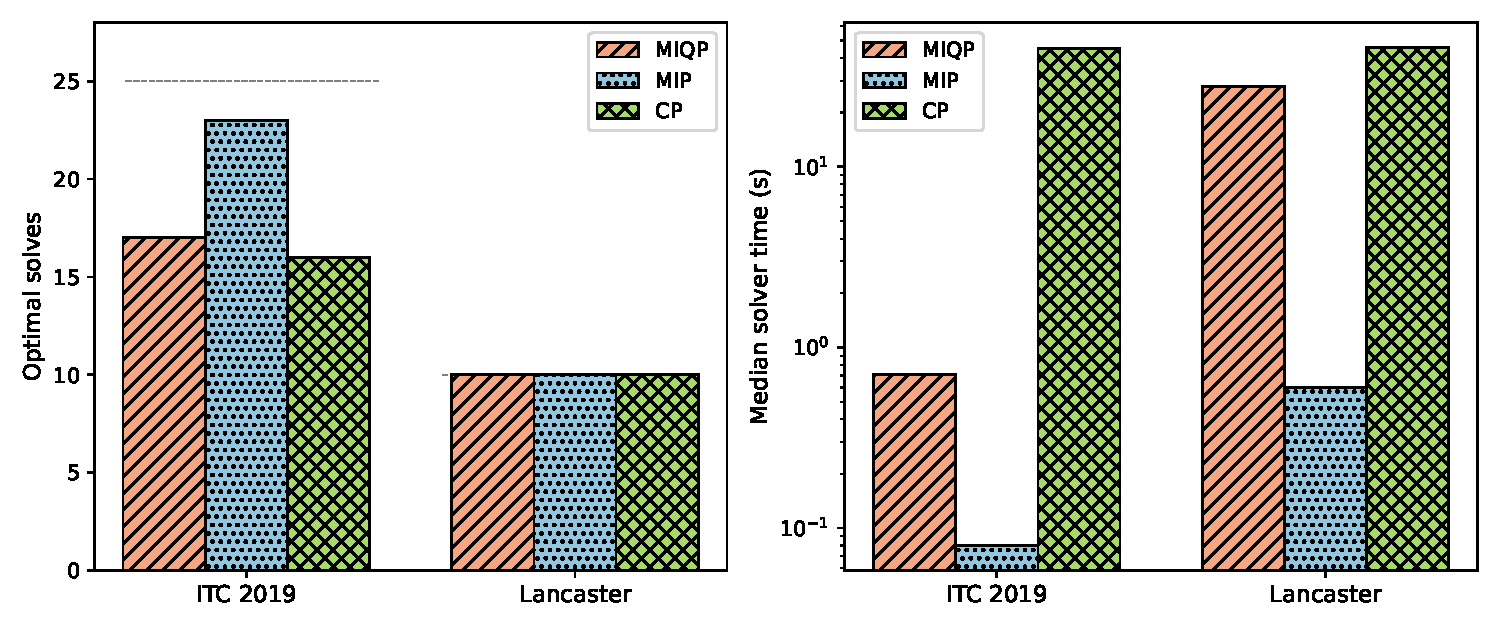
\includegraphics[width=0.98\linewidth]{figures/section42_runtime_summary.pdf}
\caption{Optimal solve counts and median solver runtimes for the representative configurations reported in Table~\ref{tab:results-overview}. The runtime panel uses a logarithmic scale.}
\label{fig:results-overview}
\end{figure}

\begin{figure}[t]
\centering
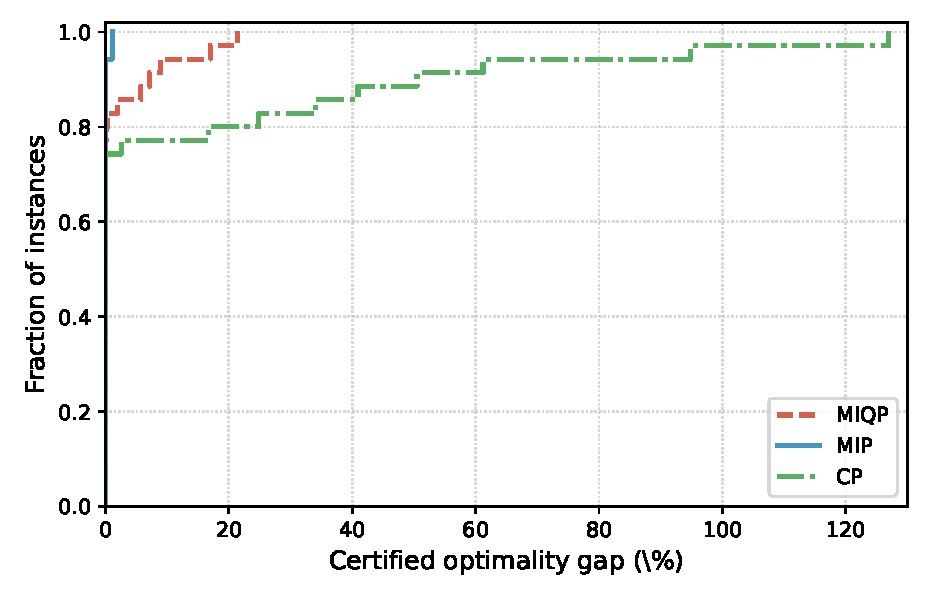
\includegraphics[width=0.65\linewidth]{figures/section42_performance_profile.pdf}
\caption{Empirical CDF of the certified optimality gap after 300 seconds for the MIQP, MIP, and CP formulations on the representative block (light preprocessing; capacity-dominance cuts off; biclique strengthening on, except ITC-MIQP which uses the weaker pairwise distance model). The $x$-axis spans $0\%$ to $130\%$ and each curve reports the fraction of the 35 benchmark instances with a certified gap at most $x$, reaching its ceiling at $1$ once $x$ exceeds the worst case or at $(n - k)/n$ if $k$ of the $n$ runs returned no incumbent.}
\label{fig:performance_profile}
\end{figure}

\begin{figure}[t]
\centering
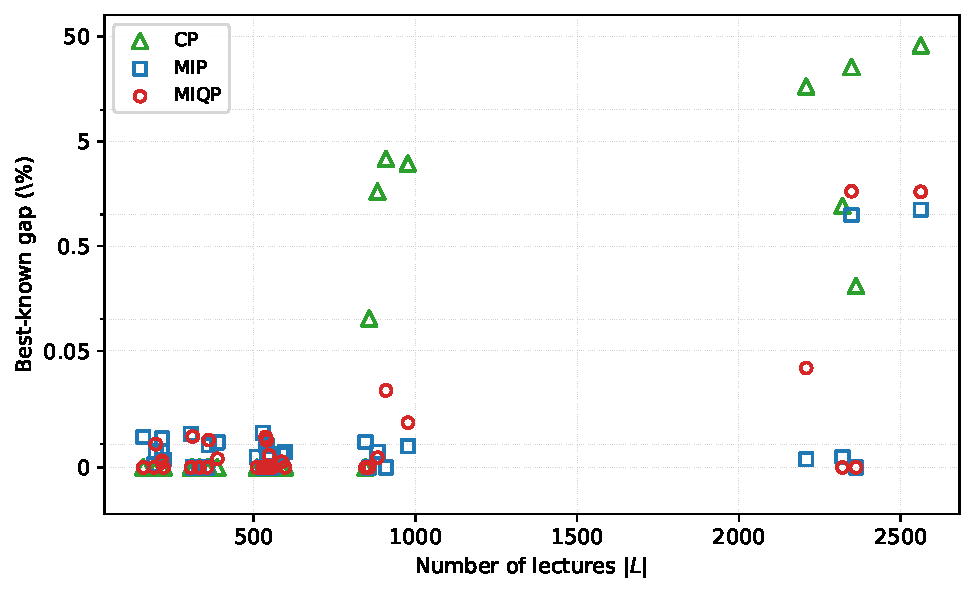
\includegraphics[width=0.78\linewidth]{figures/section_appendix_bkgap_scatter.pdf}
\caption{Best-known gap $\mathrm{bk}\% = 100(z - LB^\star)/LB^\star$ after 300 seconds plotted against the number of lectures $|L|$ for the 35 representative instances. Each instance contributes three markers, one per formulation; the $y$-axis is shown on a symmetric-log scale with a linear band of width~$0.05$ around the origin, and MIQP and MIP markers are jittered horizontally by a small random amount to disambiguate overlapping zeros.}
\label{fig:bkgap-scatter}
\end{figure}

\begin{figure}[t]
\centering
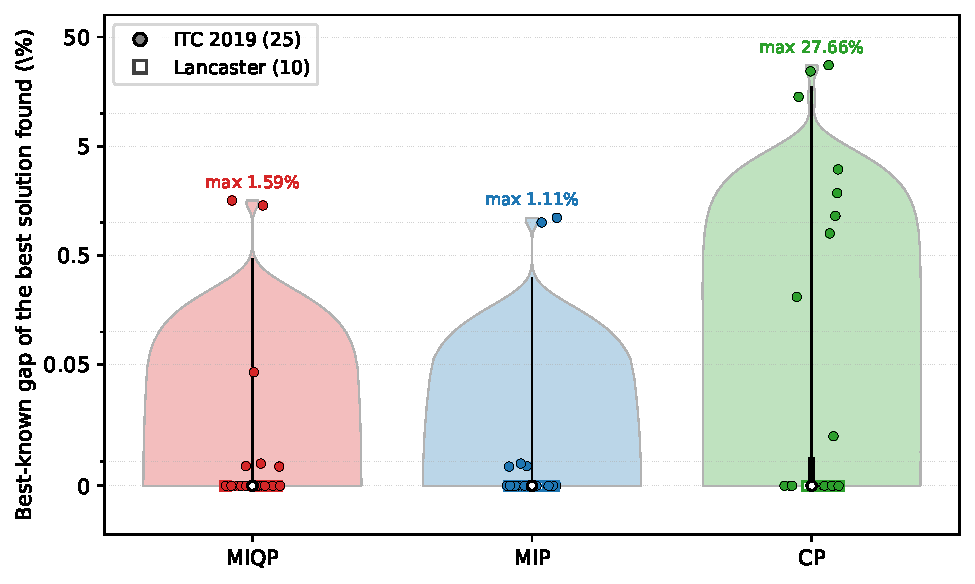
\includegraphics[width=0.72\linewidth]{figures/section42_gap_dispersion.pdf}
\caption{Distribution across the 35 benchmark instances of the best-known gap $\mathrm{bk}\% = 100 (z_{i,f}^{\star} - LB^{\star}_i) / LB^{\star}_i$ of the best solution each formulation found, where $z_{i,f}^{\star}$ is the smallest objective obtained by formulation $f$ on instance $i$ over the eight cut/preprocess settings and $LB^{\star}_i$ is the best known lower bound for instance $i$ across every exact and root run. Filled circles mark ITC instances, open squares mark Lancaster instances; white dots mark medians, thick vertical bars mark interquartile ranges, and thin whiskers span the $[5\%,95\%]$ range. The $y$-axis uses a symmetric-log scale with a linear band of width~$0.05$ around the origin.}
\label{fig:gap-dispersion}
\end{figure}


Two broad conclusions are clear from Table~\ref{tab:results-overview}, Figure~\ref{fig:results-overview}, and the Dolan--Mor\'e performance profile in Figure~\ref{fig:performance_profile}. First, the compact linearized MIP is the most robust exact formulation on this benchmark. On the 25 ITC-derived instances it solves 23 to proven optimality within the 300-second limit, compared with 17 for the MIQP model and 16 for CP-SAT. On the 10 Lancaster instances all three formulations solve every instance, but the MIP model is by far the fastest: its median solver runtime is about $0.6$ seconds, compared with roughly $28$ seconds for MIQP and $46$ seconds for CP-SAT. This dominance is clearly visualized by the MIP curve strictly dominating both MIQP and CP-SAT in the performance profile.

Second, all three methods obtain incumbents throughout the campaign: every one of the 840 exact runs returns a feasible solution. The real difference lies in proof of optimality and in the quality of the final incumbents. This is reflected in the gap columns. On the harder ITC days, CP-SAT ends with a mean proved gap of $18.10\%$ and a mean best-known gap of $3.70\%$, whereas the representative MIP block already reaches $0.09\%$ and $0.09\%$, respectively. The representative MIQP block also stays close to the best available bounds, with a mean best-known gap of only $0.14\%$. The ``Max proved gap'' column reveals the tail behaviour: the worst-case MIP gap is only $1.11\%$ (on \texttt{pu-proj-fal19\_week6\_day3}), whereas the worst-case MIQP and CP-SAT gaps reach $21.45\%$ and $126.94\%$, respectively, both on the hardest Purdue instances. These tails are visually formalized by the empirical CDF of certified gaps in Figure~\ref{fig:performance_profile}, where the MIP curve already hits $33/35$ at $0\%$ gap and captures $100\%$ of instances by the $1.11\%$ mark, whereas the MIQP and CP curves do not close $100\%$ of instances until the $21.45\%$ and $126.94\%$ marks, respectively. Figure~\ref{fig:bkgap-scatter} stratifies these aggregate statistics by instance size: MIP and MIQP points cluster at or near~$0\%$ across the full size range, CP points coincide with them on every \texttt{agh}, \texttt{muni-pdf}, \texttt{muni-pdfx}, and Lancaster instance, and the only visible spread in either axis occurs on the largest \texttt{pu-d9} and \texttt{pu-proj} days, where CP best-known gaps fan out to between~$1$ and~$41\%$ and MIQP occasionally trails MIP by a percentage point or two. In other words, the Section~\ref{sec:numerical-experiments} ranking between formulations is driven almost entirely by the largest dense instances, and the two formulation families are statistically indistinguishable on the remaining twenty-six benchmark days.

Figure~\ref{fig:gap-dispersion} summarizes the 35 \emph{best} solutions each formulation produces across the eight cut/preprocess settings: for each instance $i$ and formulation $f$ we take the smallest objective $z^{\star}_{i,f}$ found by $f$ on $i$ and report its gap $(z^{\star}_{i,f}-LB^{\star}_i)/LB^{\star}_i$ against the globally best known lower bound. This isolates the primal quality the user would observe in a production deployment that, for each (family, formulation) combination, simply runs the best configuration. The three distributions all have median~$0\%$, and both MIP and MIQP have empty interquartile ranges, so their medians and $75$\textsuperscript{th} percentiles coincide at zero. MIP is slightly tighter than MIQP (mean $0.061\%$ vs $0.088\%$; max $1.11\%$ vs $1.59\%$; five vs six instances with a strictly positive gap), but the two are statistically indistinguishable. CP is noticeably more dispersed: mean $2.09\%$, standard deviation $6.46$pp, max $27.66\%$, and nine out of $35$ instances still carry a positive best-known gap. Every nonzero CP point sits on one of the four largest \texttt{pu-d9} or \texttt{pu-proj} days; every ITC \texttt{agh}, \texttt{muni-pdf}, \texttt{muni-pdfx} day and every Lancaster day appears at the origin of every violin, confirming that the formulation ranking is determined entirely by the hardest dense instances and that on the remaining twenty-six days the three formulations are primal-equivalent.

The main driver of this performance difference is the biclique-style distance strengthening. Table~\ref{tab:root-gap} and Figure~\ref{fig:root-gap} show its effect on the root relaxation of the linearized model under the same light-preprocessing, no-capacity-dominance setting. Here we report the \emph{root shortfall}, namely the relative gap between the root lower bound and $LB^\star$. On the ITC instances, the mean root shortfall drops from $5.76\%$ for the weaker pairwise model to $0.09\%$ for the biclique-enhanced model. On the Lancaster instances, the corresponding reduction is from $20.67\%$ to $0.01\%$. The time needed to compute the root bound also decreases sharply: the median root solver time drops from about $1.9$ to $0.09$ seconds on ITC and from about $55$ to $0.6$ seconds on Lancaster.

\begin{table}[t]
\centering
\scriptsize
\begin{tabular}{@{}lrrrr@{}}
\hline
Source & Weak shortfall (\%) & Strong shortfall (\%) & Weak root time (s) & Strong root time (s) \\
\hline
ITC 2019 & 5.76 & 0.09 & 1.95 & 0.09 \\
Lancaster & 20.67 & 0.01 & 55.25 & 0.62 \\
\hline
\end{tabular}
\caption{Root-bound quality of the linearized model under light preprocessing and without capacity-dominance cuts. The shortfall is measured against the best-known lower bound $LB^\star$. Root solver times are reported as medians over the instance set. ``Weak'' denotes the weaker pairwise distance model used as the baseline in the root experiments, and ``Strong'' denotes the biclique-enhanced distance model.}
\label{tab:root-gap}
\end{table}

\begin{table}[t]
\centering
\scriptsize
\setlength{\tabcolsep}{5pt}
\begin{tabular}{@{}lccc rrrr@{}}
\hline
Formulation & PP & Bic & Dominance & \makecell{Mean best-known\\gap (\%)} & \makecell{Mean provable\\gap (\%)} & \#\,Opt. & \#\,BK \\
\hline
MIQP & none  & off & off & 0.10 & 1.63 & 25 & 32 \\
MIQP & none  & off & on  & 0.10 & 1.59 & 26 & 30 \\
MIQP & none  & on  & off & --   & --   & 27 & 27 \\
MIQP & none  & on  & on  & --   & --   & 27 & 27 \\
MIQP & light & off & off & 0.10 & 1.79 & 26 & 31 \\
MIQP & light & off & on  & 0.10 & 1.57 & 26 & 30 \\
MIQP & light & on  & off & --   & --   & 27 & 27 \\
MIQP & light & on  & on  & --   & --   & 28 & 28 \\
\hline
MIP & none  & off & off & 3.14 & 11.04 & 16 & 21 \\
MIP & none  & off & on  & 3.47 & 11.43 & 16 & 20 \\
MIP & none  & on  & off & 0.06 & 0.07  & 33 & 33 \\
MIP & none  & on  & on  & 0.06 & 0.08  & 32 & 33 \\
MIP & light & off & off & 5.13 & 13.36 & 16 & 21 \\
MIP & light & off & on  & 3.67 & 11.59 & 16 & 21 \\
MIP & light & on  & off & 0.06 & 0.06  & 33 & 35 \\
MIP & light & on  & on  & 0.06 & 0.06  & 32 & 34 \\
\hline
CP & none  & off & off & 2.60 & 9.83  & 26 & 26 \\
CP & none  & off & on  & 3.46 & 13.65 & 25 & 25 \\
CP & none  & on  & off & 2.63 & 12.92 & 26 & 26 \\
CP & none  & on  & on  & 3.87 & 17.39 & 26 & 26 \\
CP & light & off & off & 2.56 & 9.83  & 26 & 26 \\
CP & light & off & on  & 2.84 & 11.77 & 25 & 25 \\
CP & light & on  & off & 2.64 & 12.93 & 26 & 26 \\
CP & light & on  & on  & 3.70 & 16.49 & 26 & 26 \\
\hline
\end{tabular}
\caption{Per-(formulation, cut/preprocess-combination) statistics across the 35 benchmark instances under the 300-second time limit. ``PP'' is compatibility preprocessing (\emph{light} or \emph{none}); ``Bic'' toggles the biclique distance cuts; ``Dominance'' toggles the Chv\'atal--Gomory capacity-dominance cuts. ``Mean best-known gap'' averages $(z - LB^\star)/LB^\star$ and ``Mean provable gap'' averages $(z - LB)/LB$ with the run's own lower bound $LB$. Both averages are replaced by ``--'' whenever at least one of the $35$ instances returned \emph{no incumbent} (solver proved a valid lower bound but produced no feasible solution inside the time limit, so the per-instance gap is undefined and the cross-instance mean would be misleading). All four MIQP biclique-on rows trigger this rule because Gurobi's nonlinear branch-and-bound fails to return a feasible solution on three to five of the hardest Purdue days; every CP-SAT run, by contrast, returned both an incumbent and a positive lower bound on every instance, so the CP rows never take a ``--''. ``\#\,Opt.'' is the number of instances solved to proven optimality (status \textsc{optimal}); ``\#\,BK'' is the number of instances on which the run tied the globally best incumbent objective found anywhere in the factorial.}
\label{tab:factorial-per-combo}
\end{table}

Table~\ref{tab:factorial-per-combo} isolates each of the three levers. For the \emph{linearized MIP} the biclique distance cuts are the decisive lever: enabling them triples the optimal count from $16$ to $32$--$33$ (out of $35$), raises the best-known count from $20$--$21$ to $33$--$35$, and collapses the mean best-known gap from the $3$--$5\%$ range to $0.06\%$ regardless of the other two switches, with the mean provable gap dropping from above $11\%$ to at most $0.08\%$. Preprocessing and the capacity-dominance cuts are essentially neutral on top of biclique: the four MIP rows with biclique on are statistically indistinguishable on every column. For the \emph{MIQP} the picture is inverted. Without biclique, every MIQP combination reaches a mean best-known gap of $0.10\%$ and a mean provable gap of $1.57$--$1.79\%$ while returning an incumbent on every one of the $35$ instances. Turning biclique on, by contrast, makes Gurobi's nonlinear branch-and-bound drop the incumbent on three to five of the hardest Purdue instances in every one of the four biclique-on combinations, which leaves both the mean provable gap and the mean best-known gap undefined in the table (entries ``--''); on the instances that do return an incumbent, $\#\,$BK stays at $27$--$28$ rather than improving. Preprocessing and the capacity-dominance cuts amplify rather than mitigate this degradation on MIQP, because they interact with the already fragile bilinear relaxation instead of helping it. For \emph{CP-SAT} none of the three levers moves the numbers much: the best-known gap sits in a narrow $2.56$--$3.87\%$ band, both the optimal count and the best-known count oscillate between $25$ and $26$, so CP-SAT is essentially indifferent to the modeling choices and benefits most from primal heuristics inside the solver rather than from the additional inequalities. The Lancaster instances are saturated by every CP and MIQP combination and by every MIP combination with biclique on, so the dispersion in Table~\ref{tab:factorial-per-combo} is driven almost entirely by the 25 ITC days, and in particular by the five largest Purdue instances. The practical upshot is that a production deployment should pair each formulation with its dominating combination, namely light preprocessing with biclique on and capacity cuts off for MIP, any biclique-off combination for MIQP, and any combination with the capacity cuts off for CP-SAT; these are the per-formulation best settings used in the representative block of Table~\ref{tab:results-overview} and in the dispersion summary of Figure~\ref{fig:gap-dispersion}.

\begin{figure}[t]
\centering
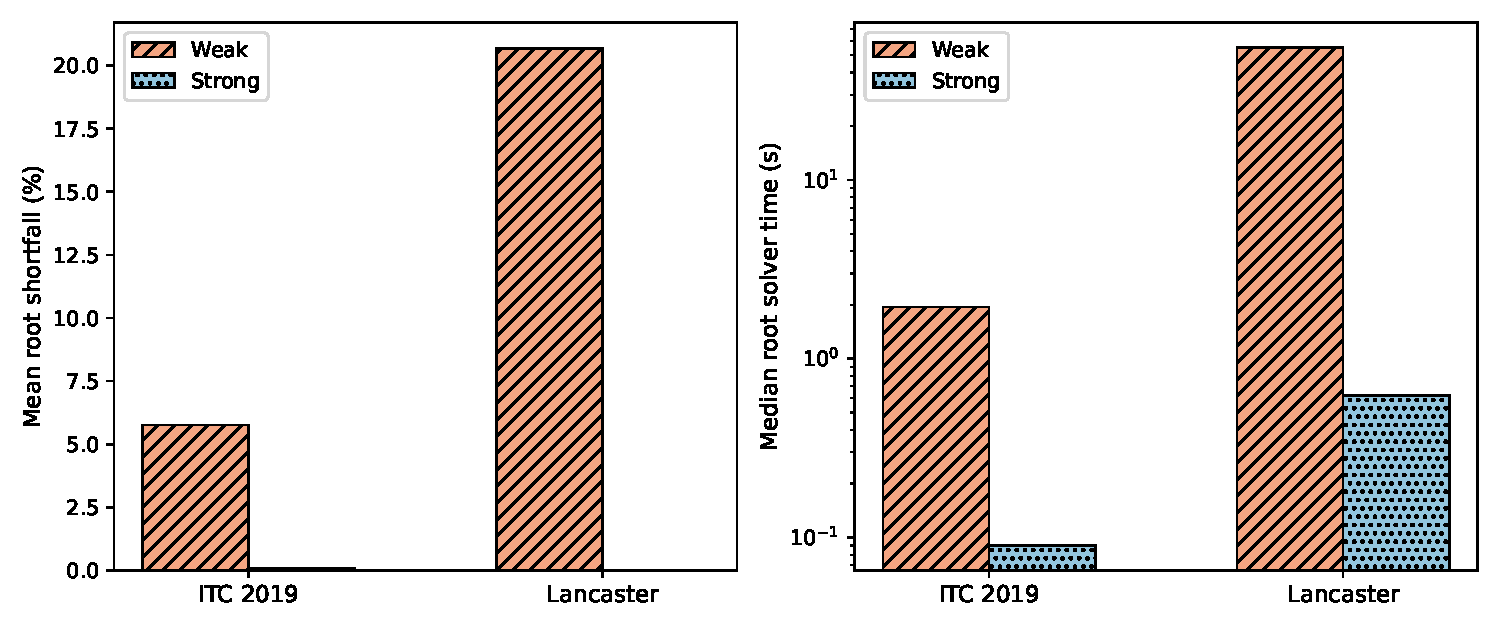
\includegraphics[width=0.98\linewidth]{figures/section42_root_summary.pdf}
\caption{Mean root shortfalls and median root solver times for the weaker and strongest linearized distance models. The runtime panel uses a logarithmic scale, matching the convention of Figure~\ref{fig:results-overview}.}
\label{fig:root-gap}
\end{figure}

The exact MIP results mirror the root-bound picture. On the ITC instances, the representative light-preprocessed MIP block improves from 16 optimal solves under the weaker distance model to 23 under the biclique-enhanced one, while the mean best-known gap drops from $7.14\%$ to $0.09\%$. On Lancaster, the weak MIP times out on all ten instances within the 300-second limit, whereas the biclique-enhanced variant solves all ten to proven optimality in under a second of median runtime. The CP formulation also benefits from stronger distance reasoning on Lancaster, where its median solver runtime falls from about $75$ to about $46$ seconds, but its ITC improvements are much smaller. For the MIQP runs, biclique strengthening is clearly beneficial on Lancaster, where it lifts the solve count from 9/10 to 10/10 and cuts the median solver runtime from about $73$ to $28$ seconds, but is actively detrimental on the hardest ITC instances, where the nonlinear branch-and-bound under the stronger cuts sometimes fails to return any incumbent within 300 seconds and consequently inflates the mean best-known gap from $0.14\%$ to $11.98\%$ while leaving the number of proved-optimal solves unchanged at 17/25.

The other two modeling improvements are useful but clearly secondary in this campaign. Light compatibility preprocessing removes on average only $3.63\%$ of compatibility entries on the ITC instances and $1.41\%$ on the Lancaster instances, so large runtime changes should not be expected from preprocessing alone. The saved runs are consistent with that expectation: preprocessing usually yields a modest speed-up, but it does not alter the qualitative ranking between formulations.

The capacity-dominance inequalities likewise have only a limited aggregate effect. To isolate their contribution we repeated the representative block of Table~\ref{tab:results-overview} with the cuts enabled, keeping all other settings fixed, and report the resulting deltas in Table~\ref{tab:cap-dominance-delta}. The cuts are essentially neutral on Lancaster: every instance was already solved to proven optimality without them, so neither the optimal count nor the best-known gap moves, and the median runtime shifts by at most $1.4$~seconds in either direction. On ITC they are a net negative for the MIP and CP formulations. They flip \texttt{pu-d9-fal19\_week2\_day3} from an optimal solve in about $263$~seconds to a MIP time-out, leaving the other MIP solves essentially unchanged, and they noticeably worsen the CP-SAT block: the mean solver-certified gap rises from $18.10\%$ to $23.09\%$, the mean best-known gap from $3.70\%$ to $5.18\%$, and the median CP-SAT runtime grows from $45$ to $75$~seconds, all without closing any additional instance. The ITC MIQP block is the closest to neutral: the cuts tighten the mean solver-certified gap from $2.51\%$ to $2.19\%$, but the mean best-known gap ticks up by $0.01$~percentage points and the solve count is unchanged, so the certified-gap improvement reflects a marginally tighter lower bound rather than a better incumbent. The cut generation itself is cheap, taking at most $65$~milliseconds per run on the largest Purdue instances, so the observed slowdowns come from the interaction between the extra inequalities and the solvers' branching, not from cut preparation. Taken together, the results suggest a clear hierarchy among the three improvements: biclique strengthening is the dominant source of bound improvement and exact-solver speed, compatibility preprocessing is a consistently mild positive, and the Chv\'atal--Gomory capacity-dominance cuts provide no measurable benefit on the 35 real-world instances studied here and should be disabled by default on this benchmark.

\begin{table}[t]
\centering
\scriptsize
\begin{tabular}{@{}llrrrr@{}}
\hline
Source & Formulation & $\Delta$Optimal & \makecell{$\Delta$Mean best-known\\gap (pp)} & \makecell{$\Delta$Median\\time (s)} & \makecell{Cut gen.\\time (s)} \\
\hline
ITC 2019 & MIQP & $+0$ & $+0.01$ & $+0.00$ & $0.061$ \\
ITC 2019 & MIP  & $-1$ & $+0.00$ & $+0.01$ & $0.065$ \\
ITC 2019 & CP   & $+0$ & $+1.48$ & $+29.94$ & $0.062$ \\
Lancaster & MIQP & $+0$ & $+0.00$ & $-0.09$ & $0.032$ \\
Lancaster & MIP  & $+0$ & $+0.00$ & $+0.02$ & $0.032$ \\
Lancaster & CP   & $+0$ & $+0.00$ & $+1.44$ & $0.032$ \\
\hline
\end{tabular}
\caption{Ceteris paribus effect of enabling capacity-dominance cuts, measured as the difference between the representative block of Table~\ref{tab:results-overview} (cuts off) and the same block with cuts on. Positive $\Delta$Optimal indicates more proved-optimal solves; positive $\Delta$Median time indicates a slower median runtime. Units of the gap delta are percentage points.}
\label{tab:cap-dominance-delta}
\end{table}


\section{Conclusions and future research}
\label{sec:conclusions}

This paper studied the \emph{lecture-hall assignment problem} that arises once a weekly timetable is fixed and student enrollments are known. The problem asks to assign each scheduled lecture to a feasible hall, respecting capacity and interval-overlap constraints, so as to minimize the total walking effort induced by students moving between consecutive lectures. This quadratic objective, driven by the product of shared enrollments and hall-to-hall distances, is absent from most of the timetabling and hall-allocation literature and yet captures a first-order operational concern at real universities, where long between-class walks generate late arrivals and place a disproportionate burden on students with mobility needs.

Our main contributions are fourfold. First, on the modeling side, we formally isolated the post-timetabling hall assignment layer from the broader university course timetabling problem and proved that, even in a restricted single-day two-block setting with identical capacities and full compatibility, the decision version is NP-complete and every approximation lower bound for the quadratic assignment problem carries over. This places the problem squarely in the QAP complexity landscape while clarifying that the usual interval-scheduling relaxations are insufficient to capture its difficulty. Second, we developed three exact formulations, a bilinear MIQP, a compact linearized MIP with one continuous distance variable per successor pair, and a CP-SAT formulation based on integer hall-assignment variables, all of which share the same feasible region and decompose by day. Third, we introduced three problem-specific modeling improvements that can be layered on top of any of the three formulations: an easy-to-separate family of \emph{biclique distance cuts} that dominates the basic pairwise linking inequalities and exploits the sparsity of lecture-hall compatibilities, a family of Chv\'atal--Gomory \emph{capacity-dominance} inequalities that combine clique-overlap constraints with hall-capacity thresholds, and a safe fixed-point \emph{compatibility-preprocessing} procedure. We also showed that the framework extends to standard timetabling side constraints such as hard and soft \emph{SameRoom} and \emph{SameAttendees}, for which the biclique construction again delivers stronger aggregated inequalities. Fourth, we conducted an extensive computational study on 35 daily instances derived from five large ITC~2019 benchmarks and from a 2023 institutional dataset at Lancaster University, totaling 840 exact runs under a 300-second time limit.

The numerical results point to a clear hierarchy among the proposed enhancements. The compact linearized MIP is the most robust exact formulation on the benchmark, solving 23 of the 25 ITC daily instances and all 10 Lancaster instances to proven optimality within the time limit, and achieving an average best-known gap of $0.09\%$ on ITC and $0.00\%$ on Lancaster in the representative block. Biclique strengthening is the dominant single modeling device: it reduces the mean root-relaxation shortfall of the linearized model from $5.76\%$ to $0.09\%$ on ITC instances and from $20.67\%$ to $0.01\%$ on Lancaster instances, and lifts MIP optimal solves from 16/25 to 23/25 on ITC while turning the weak Lancaster MIP, which times out on every instance, into a model that solves all ten in under a second of median runtime. In contrast, light compatibility preprocessing contributes a consistent modest speed-up across all configurations, while the Chv\'atal--Gomory capacity-dominance cuts, although theoretically sound, provide no measurable benefit on the 35 real-world instances studied here: they are essentially neutral for MIQP and for every Lancaster configuration, and net negative for the MIP and CP-SAT formulations on ITC. The CP-SAT formulation produces strong incumbents but is consistently slower at proving optimality, and the MIQP formulation is competitive on easier instances but loses ground on the hardest Purdue days, where the nonlinear branch-and-bound under stronger cuts sometimes fails to return any incumbent within the time limit.

Taken together, these findings suggest that realistic lecture-hall assignment problems from both a competition-grade benchmark and an institutional dataset can be solved to optimality or near-optimality within minutes by off-the-shelf MIP technology once the biclique structure of the quadratic walking term is exploited. From a practical standpoint, this places the proposed framework within reach of operations offices that are already comfortable with mathematical-programming software, and it complements the multi-objective evolutionary approaches that target the closely related but broader hall-allocation problem \citep{roomalloc2026}.

Several directions for future research appear promising. On the algorithmic side, the present biclique inequalities are separated in a static, structural manner; it would be natural to study their polyhedral strength more formally, identify classes under which they are facet-defining, and develop a dynamic separation routine embedded in a branch-and-cut scheme. Complementing this, dedicated Lagrangian or convex quadratic relaxations of the walking term, along the lines of \citet{anstreicher2003} and \citet{zhao1998}, may yield even tighter bounds on the hardest instances, and combining the linearized MIP with tabu-style heuristics inspired by \citet{taillard1991} could provide high-quality warm starts for very large instances. A second direction is to relax the assumption of a fully fixed timetable and allow limited schedule adjustments, such as swapping two lectures of the same course between adjacent time slots, which would couple the hall-assignment decision with light timetable repair while preserving much of the structural decomposition by day. Third, a rich class of robust and stochastic extensions becomes interesting once one recognizes that enrollments, disability-related weights, and hall availability are often uncertain at the time of assignment; two-stage stochastic formulations that choose a hall assignment before enrollment realization, together with appropriate scenario-based bounds, would be a natural next step. Fourth, the framework could be embedded in a digital-twin or decision-support system for campus mobility, jointly accounting for elevator and stair bottlenecks, weather and season effects on outdoor walking, and accessibility constraints for students with disabilities; the linear assignment-penalty extension already accommodates such weightings. Finally, the multi-criteria structure explored by \citet{roomalloc2026} and the hybrid-teaching dimension emphasized by \citet{davison2025} remain attractive directions: combining their broader objective landscape with the exact-optimization machinery proposed here may yield decision-support tools that are both provably optimal with respect to a primary walking objective and explicitly Pareto-aware across secondary criteria.


\bibliographystyle{plainnat}
\bibliography{refs}
\appendix

\section{Detailed per-instance numerical results}
\label{app:per-instance}

This appendix reports, for each of the 35 real-world benchmark instances used in
Section~\ref{sec:numerical-experiments}, the per-instance counterparts of the
aggregate numbers in Tables~\ref{tab:results-overview} and~\ref{tab:root-gap}.
Tables~\ref{tab:app-exact-itc} and~\ref{tab:app-exact-lan} give the exact-solve
results for the three formulations on the representative configuration (light
compatibility preprocessing, no capacity-dominance cuts, biclique strengthening
enabled except for the ITC-MIQP column, which uses the weaker pairwise distance
model for the reasons discussed in Section~\ref{sec:numerical-experiments}).
Tables~\ref{tab:app-root-itc} and~\ref{tab:app-root-lan} give the corresponding
root-relaxation results for the weak pairwise and the strong biclique-enhanced
distance models.
Each exact row reports, per formulation, the final incumbent objective value,
the solver-certified optimality gap (\%), the best-known gap (\%), and the
solver runtime (s). The best-known gap is computed against the global
$LB^\star$ column, $\mathrm{bk}\% = 100 (z - LB^\star)/LB^\star$, and it
coincides with the certified gap whenever the run attained $LB^\star$ on its
own, as is the case on every ITC \texttt{agh}, \texttt{muni-pdf},
\texttt{muni-pdfx} instance and on every Lancaster instance in the
representative block.
A dagger~($^\dagger$) marks runs that hit the 300-second time limit with
the solver still reporting \textsc{time\_limit} (non-optimal termination
but the certified gap can still be computed from the final LB and UB);
a double dagger~($^\ddagger$) marks CP-SAT runs that hit the time limit
with status \textsc{feasible} rather than \textsc{optimal}, meaning
CP-SAT returned an incumbent and a valid but loose lower bound that was
not tight enough to close the gap inside the time budget. In every run
reported in this appendix the solver returned a positive lower bound;
the gap columns are therefore always well-defined.
The column $LB^\star$ is the best lower bound obtained by any method for that
instance, and serves as the reference point for the shortfall columns in the
root tables.
The per-instance patterns mirror the aggregate summary: the linearized MIP
closes the gap on essentially every instance, the quadratic MIP also stays
close to $LB^\star$ once the ITC-MIQP exception is taken into account, and
CP-SAT closes all Lancaster instances but struggles on the large Purdue
instances. On the root relaxations, enabling biclique distance
strengthening reduces the shortfall to within a fraction of a percent on
almost every instance and turns a solver that times out on many instances
into one that returns a certified root bound in a few tenths of a second.

\begin{table}[ht]
\centering
\scriptsize
\setlength{\tabcolsep}{2pt}
\begin{tabular}{@{}lrr rrrr rrrr rrrr@{}}
\hline
 & & & \multicolumn{4}{c}{MIQP} & \multicolumn{4}{c}{MIP} & \multicolumn{4}{c}{CP} \\
Instance & $|L|$ & $LB^\star$ & obj & gap\% & bk\% & t\,(s) & obj & gap\% & bk\% & t\,(s) & obj & gap\% & bk\% & t\,(s) \\
\hline
\texttt{agh w4d1} & 542 & 966 & 966 & 0.00 & 0.00 & 0.39 & 966 & 0.00 & 0.00 & 0.06 & 966 & 0.00 & 0.00 & 6.8 \\
\texttt{agh w4d2} & 558 & 649 & 649 & 0.00 & 0.00 & 0.37 & 649 & 0.00 & 0.00 & 0.06 & 649 & 0.00 & 0.00 & 9.1 \\
\texttt{agh w4d3} & 540 & 509 & 509 & 0.00 & 0.00 & 0.24 & 509 & 0.00 & 0.00 & 0.08 & 509 & 0.00 & 0.00 & 5.3 \\
\texttt{agh w4d4} & 537 & 523 & 523 & 0.00 & 0.00 & 0.39 & 523 & 0.00 & 0.00 & 0.07 & 523 & 0.00 & 0.00 & 6.3 \\
\texttt{agh w4d5} & 540 & 559 & 559 & 0.00 & 0.00 & 0.22 & 559 & 0.00 & 0.00 & 0.08 & 559 & 0.00 & 0.00 & 4.2 \\
\texttt{muni-pdf w3d1} & 217 & 85 & 85 & 0.00 & 0.00 & 0.00 & 85 & 0.00 & 0.00 & 0.00 & 85 & 0.00 & 0.00 & 0.00 \\
\texttt{muni-pdf w3d2} & 222 & 143 & 143 & 0.00 & 0.00 & 0.00 & 143 & 0.00 & 0.00 & 0.00 & 143 & 0.00 & 0.00 & 0.00 \\
\texttt{muni-pdf w3d3} & 217 & 148 & 148 & 0.00 & 0.00 & 0.00 & 148 & 0.00 & 0.00 & 0.00 & 148 & 0.00 & 0.00 & 0.00 \\
\texttt{muni-pdf w3d4} & 192 & 120 & 120 & 0.00 & 0.00 & 0.00 & 120 & 0.00 & 0.00 & 0.00 & 120 & 0.00 & 0.00 & 0.00 \\
\texttt{muni-pdf w3d5} & 159 & 306 & 306 & 0.00 & 0.00 & 0.32 & 306 & 0.00 & 0.00 & 0.03 & 306 & 0.00 & 0.00 & 2.2 \\
\texttt{muni-pdfx w12d1} & 361 & 1611 & 1611 & 0.00 & 0.00 & 0.86 & 1611 & 0.00 & 0.00 & 0.05 & 1611 & 0.00 & 0.00 & 39 \\
\texttt{muni-pdfx w12d2} & 356 & 1543 & 1543 & 0.00 & 0.00 & 0.71 & 1543 & 0.00 & 0.00 & 0.13 & 1543 & 0.00 & 0.00 & 45 \\
\texttt{muni-pdfx w12d3} & 388 & 2365 & 2365 & 0.00 & 0.00 & 1.0 & 2365 & 0.00 & 0.00 & 0.06 & 2365 & 0.00 & 0.00 & 57 \\
\texttt{muni-pdfx w12d4} & 332 & 1469 & 1469 & 0.00 & 0.00 & 0.59 & 1469 & 0.00 & 0.00 & 0.05 & 1469 & 0.00 & 0.00 & 87 \\
\texttt{muni-pdfx w12d5} & 197 & 909 & 909 & 0.00 & 0.00 & 0.53 & 909 & 0.00 & 0.00 & 0.05 & 909 & 0.00 & 0.00 & 2.6 \\
\texttt{pu-d9 w2d1} & 909 & 12301 & 12304 & 5.70 & 0.02 & 300$^\dagger$ & 12302 & 0.00 & 0.01 & 37 & 12719 & 50.50 & 3.40 & 301$^\ddagger$ \\
\texttt{pu-d9 w2d2} & 846 & 6066 & 6066 & 0.00 & 0.00 & 2.7 & 6066 & 0.00 & 0.00 & 0.61 & 6066 & 0.00 & 0.00 & 65 \\
\texttt{pu-d9 w2d3} & 977 & 12654 & 12655 & 7.15 & 0.01 & 300$^\dagger$ & 12655 & 0.00 & 0.01 & 263 & 13042 & 40.95 & 3.07 & 301$^\ddagger$ \\
\texttt{pu-d9 w2d4} & 857 & 4902 & 4902 & 0.00 & 0.00 & 15 & 4902 & 0.00 & 0.00 & 8.1 & 4907 & 2.55 & 0.10 & 300$^\ddagger$ \\
\texttt{pu-d9 w2d5} & 883 & 10944 & 10945 & 1.97 & 0.01 & 300$^\dagger$ & 10945 & 0.00 & 0.01 & 23 & 11125 & 34.08 & 1.65 & 301$^\ddagger$ \\
\texttt{pu-proj w6d1} & 2348 & 24076 & 24479 & 16.97 & 1.67 & 300$^\dagger$ & 24317 & 1.10 & 1.00 & 300$^\dagger$ & 30195 & 94.82 & 25.42 & 302$^\ddagger$ \\
\texttt{pu-proj w6d2} & 2362 & 10078 & 10078 & 0.39 & 0.00 & 300$^\dagger$ & 10078 & 0.00 & 0.00 & 10 & 10099 & 24.82 & 0.21 & 300$^\ddagger$ \\
\texttt{pu-proj w6d3} & 2562 & 24382 & 24781 & 21.45 & 1.64 & 300$^\dagger$ & 24652 & 1.11 & 1.11 & 300$^\dagger$ & 34347 & 126.94 & 40.87 & 302$^\ddagger$ \\
\texttt{pu-proj w6d4} & 2320 & 9980 & 9980 & 0.10 & 0.00 & 300$^\dagger$ & 9980 & 0.00 & 0.00 & 3.9 & 10101 & 16.68 & 1.21 & 300$^\ddagger$ \\
\texttt{pu-proj w6d5} & 2208 & 21373 & 21385 & 8.92 & 0.06 & 300$^\dagger$ & 21373 & 0.00 & 0.00 & 221 & 24920 & 61.19 & 16.60 & 302$^\ddagger$ \\
\hline
\end{tabular}
\caption{Per-instance exact-solve results on the 25 ITC~2019 benchmark days.
All rows use light compatibility preprocessing and no capacity-dominance cuts;
the MIP and CP columns use biclique distance strengthening, whereas the MIQP
column uses the weaker pairwise distance model for the reasons discussed in
Section~\ref{sec:numerical-experiments}. Sub-column ``gap\%'' is the
solver-certified gap against that run's own lower bound, and ``bk\%'' is the
best-known gap $(z-LB^\star)/LB^\star$ against the global reference in the
third column. Instance names abbreviate
\texttt{agh-fal17}, \texttt{muni-pdf-spr16c}, \texttt{muni-pdfx-fal17},
\texttt{pu-d9-fal19}, and \texttt{pu-proj-fal19}; week and day indices are
encoded as \texttt{wXdY}. $^\dagger$~time limit reached with status
\textsc{time\_limit}; $^\ddagger$~CP-SAT time-limit termination with
status \textsc{feasible} (incumbent returned and lower bound valid but
too loose to certify optimality inside the $300$-second budget).}
\label{tab:app-exact-itc}
\end{table}

\begin{table}[ht]
\centering
\scriptsize
\setlength{\tabcolsep}{2pt}
\begin{tabular}{@{}lrr rrrr rrrr rrrr@{}}
\hline
 & & & \multicolumn{4}{c}{MIQP} & \multicolumn{4}{c}{MIP} & \multicolumn{4}{c}{CP} \\
Instance & $|L|$ & $LB^\star$ & obj & gap\% & bk\% & t\,(s) & obj & gap\% & bk\% & t\,(s) & obj & gap\% & bk\% & t\,(s) \\
\hline
\texttt{lancs t1 w13d1} & 528 & 4319 & 4319 & 0.00 & 0.00 & 22 & 4319 & 0.00 & 0.00 & 0.37 & 4319 & 0.00 & 0.00 & 57 \\
\texttt{lancs t1 w13d2} & 528 & 2585 & 2585 & 0.00 & 0.00 & 14 & 2585 & 0.00 & 0.00 & 0.27 & 2585 & 0.00 & 0.00 & 43 \\
\texttt{lancs t1 w13d3} & 306 & 1650 & 1650 & 0.00 & 0.00 & 8.5 & 1650 & 0.00 & 0.00 & 0.14 & 1650 & 0.00 & 0.00 & 10 \\
\texttt{lancs t1 w13d4} & 587 & 2848 & 2848 & 0.00 & 0.00 & 31 & 2848 & 0.00 & 0.00 & 1.4 & 2848 & 0.00 & 0.00 & 49 \\
\texttt{lancs t1 w13d5} & 510 & 2866 & 2866 & 0.00 & 0.00 & 26 & 2866 & 0.00 & 0.00 & 0.61 & 2866 & 0.00 & 0.00 & 35 \\
\texttt{lancs t2 w28d1} & 548 & 3105 & 3105 & 0.00 & 0.00 & 43 & 3105 & 0.00 & 0.00 & 1.9 & 3105 & 0.00 & 0.00 & 62 \\
\texttt{lancs t2 w28d2} & 533 & 3944 & 3944 & 0.00 & 0.00 & 61 & 3944 & 0.00 & 0.00 & 6.8 & 3944 & 0.00 & 0.00 & 41 \\
\texttt{lancs t2 w28d3} & 312 & 1860 & 1860 & 0.00 & 0.00 & 5.5 & 1860 & 0.00 & 0.00 & 0.16 & 1860 & 0.00 & 0.00 & 13 \\
\texttt{lancs t2 w28d4} & 597 & 2673 & 2673 & 0.00 & 0.00 & 30 & 2673 & 0.00 & 0.00 & 1.8 & 2673 & 0.00 & 0.00 & 57 \\
\texttt{lancs t2 w28d5} & 546 & 2772 & 2772 & 0.00 & 0.00 & 48 & 2772 & 0.00 & 0.00 & 0.58 & 2772 & 0.00 & 0.00 & 68 \\
\hline
\end{tabular}
\caption{Per-instance exact-solve results on the 10 Lancaster~2022/23 benchmark
days. All rows use the representative configuration with biclique distance
strengthening enabled for all three formulations. Sub-column ``bk\%'' is the
best-known gap $(z-LB^\star)/LB^\star$ and equals the certified gap on every
row because every formulation reaches $LB^\star$. Instance names abbreviate
\texttt{lancs-yr23\_term1} and \texttt{lancs-yr23\_term2}; week and day
indices are encoded as \texttt{wXdY}.}
\label{tab:app-exact-lan}
\end{table}

\begin{table}[ht]
\centering
\scriptsize
\setlength{\tabcolsep}{4pt}
\begin{tabular}{@{}lr rrr rrr@{}}
\hline
 & & \multicolumn{3}{c}{Weak (pairwise)} & \multicolumn{3}{c}{Strong (biclique)} \\
Instance & $LB^\star$ & LB & shortfall\% & t\,(s) & LB & shortfall\% & t\,(s) \\
\hline
\texttt{agh w4d1} & 966 & 965 & 0.10 & 0.46 & 966 & 0.00 & 0.07 \\
\texttt{agh w4d2} & 649 & 644 & 0.77 & 0.43 & 649 & 0.00 & 0.06 \\
\texttt{agh w4d3} & 509 & 509 & 0.00 & 0.24 & 509 & 0.00 & 0.09 \\
\texttt{agh w4d4} & 523 & 519 & 0.76 & 0.74 & 521 & 0.38 & 0.08 \\
\texttt{agh w4d5} & 559 & 559 & 0.00 & 0.30 & 559 & 0.00 & 0.08 \\
\texttt{muni-pdf w3d1} & 85 & 85 & 0.00 & 0.00 & 85 & 0.00 & 0.00 \\
\texttt{muni-pdf w3d2} & 143 & 143 & 0.00 & 0.00 & 143 & 0.00 & 0.00 \\
\texttt{muni-pdf w3d3} & 148 & 148 & 0.00 & 0.00 & 148 & 0.00 & 0.00 \\
\texttt{muni-pdf w3d4} & 120 & 120 & 0.00 & 0.00 & 120 & 0.00 & 0.00 \\
\texttt{muni-pdf w3d5} & 306 & 306 & 0.00 & 0.41 & 306 & 0.00 & 0.03 \\
\texttt{muni-pdfx w12d1} & 1611 & 1611 & 0.00 & 1.5 & 1611 & 0.00 & 0.05 \\
\texttt{muni-pdfx w12d2} & 1543 & 1523 & 1.30 & 2.8 & 1543 & 0.00 & 0.13 \\
\texttt{muni-pdfx w12d3} & 2365 & 2365 & 0.00 & 1.9 & 2365 & 0.00 & 0.06 \\
\texttt{muni-pdfx w12d4} & 1469 & 1469 & 0.00 & 2.4 & 1469 & 0.00 & 0.06 \\
\texttt{muni-pdfx w12d5} & 909 & 909 & 0.00 & 0.88 & 909 & 0.00 & 0.06 \\
\texttt{pu-d9 w2d1} & 12301 & 10659 & 13.35 & 300$^\dagger$ & 12301 & 0.00 & 37 \\
\texttt{pu-d9 w2d2} & 6066 & 5951 & 1.90 & 14$^\dagger$ & 6066 & 0.00 & 0.61 \\
\texttt{pu-d9 w2d3} & 12654 & 10712 & 15.35 & 300$^\dagger$ & 12602 & 0.41 & 58$^\dagger$ \\
\texttt{pu-d9 w2d4} & 4902 & 4671 & 4.71 & 28$^\dagger$ & 4872 & 0.61 & 4.2$^\dagger$ \\
\texttt{pu-d9 w2d5} & 10944 & 9346 & 14.60 & 224$^\dagger$ & 10944 & 0.00 & 23 \\
\texttt{pu-proj w6d1} & 24076 & 17434 & 27.59 & 300$^\dagger$ & 24031 & 0.19 & 153$^\dagger$ \\
\texttt{pu-proj w6d2} & 10078 & 9269 & 8.03 & 125$^\dagger$ & 10065 & 0.13 & 10$^\dagger$ \\
\texttt{pu-proj w6d3} & 24382 & 17724 & 27.31 & 300$^\dagger$ & 24369 & 0.05 & 147$^\dagger$ \\
\texttt{pu-proj w6d4} & 9980 & 9069 & 9.13 & 144$^\dagger$ & 9980 & 0.00 & 3.9 \\
\texttt{pu-proj w6d5} & 21373 & 17282 & 19.14 & 300$^\dagger$ & 21295 & 0.36 & 48$^\dagger$ \\
\hline
\end{tabular}
\caption{Per-instance root-relaxation results for the linearized MIP on the 25
ITC~2019 benchmark days. ``Weak'' denotes the LP relaxation of the pairwise
distance model used as baseline in the root experiments; ``Strong'' denotes
the biclique-enhanced distance model. Shortfall is measured as
$(LB^\star - LB)/LB^\star$. Reported runtimes include root cut generation;
$^\dagger$~time limit reached.}
\label{tab:app-root-itc}
\end{table}

\begin{table}[ht]
\centering
\scriptsize
\setlength{\tabcolsep}{4pt}
\begin{tabular}{@{}lr rrr rrr@{}}
\hline
 & & \multicolumn{3}{c}{Weak (pairwise)} & \multicolumn{3}{c}{Strong (biclique)} \\
Instance & $LB^\star$ & LB & shortfall\% & t\,(s) & LB & shortfall\% & t\,(s) \\
\hline
\texttt{lancs t1 w13d1} & 4319 & 3460 & 19.89 & 54$^\dagger$ & 4319 & 0.00 & 0.38 \\
\texttt{lancs t1 w13d2} & 2585 & 2221 & 14.08 & 46$^\dagger$ & 2585 & 0.00 & 0.28 \\
\texttt{lancs t1 w13d3} & 1650 & 1485 & 10.00 & 22$^\dagger$ & 1650 & 0.00 & 0.15 \\
\texttt{lancs t1 w13d4} & 2848 & 2027 & 28.83 & 59$^\dagger$ & 2848 & 0.00 & 1.4 \\
\texttt{lancs t1 w13d5} & 2866 & 2363 & 17.55 & 40$^\dagger$ & 2866 & 0.00 & 0.64 \\
\texttt{lancs t2 w28d1} & 3105 & 2486 & 19.94 & 91$^\dagger$ & 3102 & 0.10 & 2.0 \\
\texttt{lancs t2 w28d2} & 3944 & 2963 & 24.87 & 64$^\dagger$ & 3944 & 0.00 & 6.9 \\
\texttt{lancs t2 w28d3} & 1860 & 1550 & 16.67 & 21$^\dagger$ & 1860 & 0.00 & 0.14 \\
\texttt{lancs t2 w28d4} & 2673 & 2047 & 23.42 & 57$^\dagger$ & 2673 & 0.00 & 1.9 \\
\texttt{lancs t2 w28d5} & 2772 & 1901 & 31.42 & 78$^\dagger$ & 2772 & 0.00 & 0.60 \\
\hline
\end{tabular}
\caption{Per-instance root-relaxation results for the linearized MIP on the 10
Lancaster~2022/23 benchmark days. Notation as in
Table~\ref{tab:app-root-itc}.}
\label{tab:app-root-lan}
\end{table}

\begin{comment}
\section{Synthetic instance generator}
The numerical study relies on a synthetic instance generator implemented in the accompanying code base. The purpose of this generator is not to reproduce one specific university in all operational details, but rather to create controlled benchmark instances that preserve the structural drivers of the lecture-hall assignment problem: heterogeneous hall sizes, fixed-time overlap patterns, cohort-based demand, sparse but meaningful successor relations, and compatibility sets that are neither trivial nor artificially restrictive. Since the problem is separable by day, every generated instance represents a single teaching day. This keeps the benchmark focused on the intrinsic daily assignment difficulty without any loss of generality relative to a weekly formulation.

The generator first creates the halls. Each hall is assigned a capacity drawn from a broad range and a location in a two-dimensional campus plane. Inter-hall distances are then obtained from scaled Euclidean distances and rounded upward to integers. This construction reflects two practical considerations. First, universities typically operate a heterogeneous stock of lecture halls and lecture halls, so uniform hall capacities would understate the assignment difficulty. Second, a geometric distance model yields a coherent metric structure, which is more realistic than an arbitrary distance matrix and better aligned with the interpretation of the objective as walking effort across campus.

Next, the generator creates a fixed lecture timetable. Let $\delta \in (0,1]$ denote the target density, interpreted as the fraction of available hall-time slots that should be occupied by lectures. The total occupied volume is therefore chosen as approximately $\delta |H||T|$, where $|T|$ is the number of time slots in the single day. This occupied volume is decomposed into lecture durations of $2$, $3$, or $4$ consecutive slots and then packed into hall-day bins. Within each bin, random idle gaps are inserted between lectures. The use of a density parameter makes the benchmark scalable in a transparent way: increasing $\delta$ simultaneously increases hall contention and the size of the overlap graph. Restricting durations to a small range of moderate lengths is also practically reasonable, since most university teaching activities are neither one-slot micro-events nor all-day blocks.

Each generated lecture is then assigned an academic identity consisting of a subject, a study year, and a compulsory/elective flag. In the current implementation, subjects are balanced across a fixed list of disciplines, study years are balanced across four cohorts, and approximately $70\%$ of lectures are designated compulsory. The balance requirement prevents degenerate instances in which one subject or one year dominates the benchmark purely by chance. More importantly, the generator imposes a cohort-overlap rule: for any fixed subject-year cohort and time slot, there may be at most one compulsory lecture, or at most two elective lectures, but not both simultaneously. This rule encodes a common curricular reality. Compulsory offerings for a cohort are usually scheduled so as not to conflict with each other, whereas a small amount of parallelism among electives is realistic and even desirable.

The implementation contains a two-level fallback mechanism to enforce these curriculum rules robustly on dense instances. First, the generator computes the maximum simultaneous lecture volume implied by the cohort system itself. With the current choice of eight subjects and four study years, there are $32$ cohorts, so the overlap rule permits at most $64$ active lectures in any slot. If the requested density would force more lecture-slots than this concurrency cap allows, the instance request is declared infeasible immediately rather than being passed to a downstream routine that would inevitably fail. Second, even when the requested density is globally feasible, a particular random packing of lecture durations into the day may still create an overly congested slot pattern or a timetable for which the greedy attribute assignment gets stuck. In that case the code first tries a small exact CP-SAT feasibility model for the balanced attribute-assignment subproblem. If that still fails, the timetable layout itself is redrawn and the process is repeated. This safeguard has a methodological purpose: hard benchmark instances should arise from the optimization problem, not from accidental inconsistencies in the synthetic curriculum generator.

After the timetable structure is fixed, the generator simulates student demand rather than drawing lecture sizes independently. This choice is important because the objective depends on shared enrollments between consecutive lectures, so generating only lecture sizes would miss the main source of quadratic coupling. The code first estimates the size of each subject-year cohort from the capacities of its compulsory offerings. Intuitively, compulsory lectures anchor the scale of a cohort better than electives do, because they are the courses that most students in the cohort are expected to attend. The generator then simulates individual student journeys through the day. Students almost always attend compulsory lectures of their own cohort, attend home-cohort electives with moderate probability, only occasionally attend previous-year electives in the same subject, and only very rarely attend electives from another subject. When several candidate electives are available, the choice is weighted by a lecture-specific popularity factor and by the remaining hidden hall capacity. This produces three desirable effects simultaneously: large core lectures emerge naturally, elective demand is split across parallels, and successor weights are concentrated on academically plausible lecture pairs rather than spread uniformly across the timetable.

The generator also introduces a latent or hidden hall for each lecture during the data-creation stage. This hidden hall is used only to shape the simulated demand and is not revealed to the optimizer as a prescribed assignment. After student journeys are simulated, lecture attendance is tightened upward toward the capacity of the hidden hall. Compulsory lectures are pushed to a higher occupancy band than electives, and lecture sizes are also kept above the next smaller capacity tier whenever possible. The practical motivation is to avoid synthetic instances in which most lectures are far smaller than the halls that can host them. Without this tightening step, the compatibility sets would often be excessively large, the capacity constraints would be weak, and the wasted-space penalty would rarely matter. The tightening procedure therefore preserves feasibility while making hall choice consequential, which is exactly the regime in which lecture-hall assignment is operationally interesting.

Finally, the benchmark data used by the optimization models are derived from the simulated attendance. For each lecture $l$, the compatibility set $H(l)$ contains all halls whose capacity is at least the final attendance of $l$. For each pair of lectures $(l_1,l_2)$, the common-student weight $c_{l_1,l_2}$ is defined by the number of simulated students who attend $l_1$ and then $l_2$ in immediately consecutive time slots on the same day. This ensures that the successor relation is sparse and behaviorally grounded: only lecture pairs that arise naturally from student schedules receive positive walking weight. In the extended objective used in the code, each compatible assignment $(l,h)$ also receives a penalty for severe under-utilization of the hall. The penalty is zero as long as at least $90\%$ of the hall is filled, and it then increases quadratically with the number of excess empty seats beyond that threshold. This reflects the practical view that assigning a lecture to a slightly oversized hall may be acceptable, whereas assigning it to a much larger hall becomes increasingly undesirable.


\end{comment}

\end{document}
